\documentclass[preprint,12pt]{elsarticle}
\usepackage{amsmath,amssymb,graphicx,booktabs,multirow,xcolor,siunitx,microtype,url}
\usepackage[ruled,vlined,linesnumbered]{algorithm2e}
\usepackage[hidelinks]{hyperref}
\usepackage{caption}
\usepackage{float}
\captionsetup{font=small}
\newcommand{\todo}[1]{\textcolor{red}{[TODO: #1]}}   % marked placeholders; search for TODO before submission
\newcommand{\nats}{\,nats}
\DeclareMathOperator{\dirn}{unit}
\DeclareMathOperator{\tr}{tr}
\journal{Information Sciences}
\setlength{\emergencystretch}{3em}

\begin{document}
\begin{frontmatter}
\title{Calibrated Ridge Maps for Token-Embedding Transplantation Across Language Models}

\author[a]{Shibdas Bhattacharya\corref{cor1}}
\ead{23dp0094@iitism.ac.in}
\author[a]{Haider Banka}
\ead{haider@iitism.ac.in}
\cortext[cor1]{Corresponding author.}
\affiliation[a]{organization={Department of Computer Science and Engineering, Indian Institute of Technology (Indian School of Mines)},city={Dhanbad},country={India}}

\begin{abstract}
Replacing the tokenizer of a pretrained language model, or adding new tokens to it, requires embeddings for tokens the model has never seen. Existing initialisations are either heuristic (subword means, FOCUS, WECHSEL) or rely on per-token sparse reconstruction (orthogonal matching pursuit, OMP). We propose a calibrated ridge map. It centres the donor and receiver embedding spaces on shared tokens and fits a closed-form ridge map from donor to receiver. It keeps only the direction of the mapped vector and sets its length by one small calibration against negative log-likelihood (NLL) on training text; no gradient is computed. We compare it with the official mergekit OMP-64, FOCUS and WECHSEL, and with our own adaptations of least squares, Procrustes and a local-regression (SALT-style) baseline, on GPT-2, OPT, Pythia and Qwen2.5 pairs from 125M to 1.5B parameters. In real vocabulary expansion, over 16 runs on PubMed and arXiv text with small receivers, ridge has a lower NLL than OMP-64 with centred inputs in all 32 paired comparisons, with small margins of 0.1 to 3.3 nats per sentence. On seven PubMed pairs up to 1.5B parameters, it is better than, or not significantly different from, each baseline in at least 13 of 14 comparisons; we report the three exceptions. For the two receivers of 1B parameters or more, every initialisation we tested, ridge included, is worse than leaving the words split. We also find that official OMP as shipped fails on GPT-2 receivers unless its inputs are centred. Building the new rows is 4 to 150 times faster than official OMP-64 on the same device with a fixed regularisation strength, because ridge time hardly depends on the number of new tokens; with a regularisation search it is up to 36 times faster, and no faster for 82 new tokens. After fine-tuning or in a frozen-feature probe, all good initialisations perform alike, so we claim no downstream advantage.
\end{abstract}

\begin{keyword}
tokenizer transplantation \sep embedding initialisation \sep vocabulary expansion \sep ridge regression \sep orthogonal matching pursuit \sep language models
\end{keyword}
\end{frontmatter}

%% ------------------------------------------------------------------
\section{Introduction}
\label{sec:intro}
A pretrained language model is tied to its tokenizer. When the tokenizer must change, the model needs embeddings for tokens it has never seen. This happens when a general model is adapted to a technical domain by adding frequent domain words as single tokens, when a model is moved to a more efficient or multilingual vocabulary, and when two models with different vocabularies must be merged, ensembled or distilled into one another \cite{goddard2024mergekit,minixhofer2024zett,mundra2024empirical}. Training new embeddings from scratch is costly, and random or mean initialisation is a weak starting point. Several \emph{gradient-free} initialisations have therefore been proposed. The simplest average the receiver embeddings of the pieces a new token splits into \cite{gee2022fvt,hewitt2021initializing}. WECHSEL and FOCUS weight existing embeddings by the similarity of auxiliary static embeddings \cite{minixhofer2022wechsel,dobler2023focus}. Orthogonal matching pursuit (OMP), now the default in the mergekit tokensurgeon tool, writes each new token as a sparse combination of shared tokens in the donor embedding space and applies the same coefficients to the receiver embeddings of those tokens \cite{goddard2025omp,goddard2024mergekit}.

OMP-style reconstruction has two properties that deserve scrutiny. It solves a separate sparse problem for every new token, whose cost grows with the number of new tokens and with the size of the shared vocabulary. It also works in the raw coordinates of the two embedding spaces, which are anisotropic and share a large common mean component \cite{ethayarajh2019contextual,mu2018allbutthetop}. We show that this matters: run exactly as shipped, the official OMP produces new rows that increase the NLL of a GPT-2 receiver by hundreds to thousands of nats, and the failure disappears when the inputs are mean-centred.

We study a simpler alternative. Instead of one sparse problem per token, we fit one linear map from the donor space to the receiver space on the shared tokens (the \emph{anchors}), in closed form with ridge regularisation \cite{hoerl1970ridge}, after centring both spaces. The map predicts a direction in the receiver space. Its length is not trusted, because ridge predictions are shrunk, but set by one calibration: the scale that minimises the NLL of the receiver on a few hundred training sentences. The method is gradient-free: no parameter of the language model is updated and no gradient is computed; the calibration only evaluates the loss.

\paragraph{Contributions} We make the following contributions, and state their limits.
\begin{enumerate}
\item \textbf{Method.} A closed-form, receiver-calibrated ridge initialiser for new token embeddings (Section~\ref{sec:method}), whose cost depends on the number of new tokens only through one matrix product.
\item \textbf{Evidence in vocabulary expansion.} In real vocabulary expansion (16 runs, four receiver--donor pairs, PubMed and arXiv text, Section~\ref{sec:realvocab}), ridge has a lower NLL than the official OMP-64 with centred inputs in all 32 paired comparisons (zero-shot and after 200 steps on the new rows), by small margins (0.1--3.3 nats per sentence), and a lower NLL than a sparse OMP-32, a mean-of-pieces baseline and, in four PubMed runs, official WECHSEL. On seven PubMed pairs from 125M to 1.5B parameters (Section~\ref{sec:scale}) it is better than, or not significantly different from, centred OMP-64, OMP-64 as shipped, least squares, Procrustes, a SALT-style local regression (our adaptation) and WECHSEL in at least 13 of 14 comparisons each; we report the three exceptions, and the finding that for the two receivers of 1B parameters or more no initialisation beats leaving the words split.
\item \textbf{A baseline failure and its repair.} Official OMP as shipped fails on GPT-2 receivers; centring its inputs repairs it. We evaluate both versions.
\item \textbf{Efficiency, measured fairly.} On the same device and dtype, the mapping step is 4--5 times faster than official OMP-64 for 82 new tokens and 131--153 times faster for 3000 with a fixed regularisation strength (Section~\ref{sec:speed}).
\item \textbf{Honest downstream and ablation results.} After fine-tuning and in a frozen-feature probe with Holm-corrected tests, strong initialisations are statistically indistinguishable, so we make no downstream claim. Ablations show which components matter (Section~\ref{sec:ablation}).
\end{enumerate}

\section{Related work}
\label{sec:related}
\paragraph{Heuristic initialisation} Initialising a new token with the mean of the receiver embeddings of its pieces is the common default \cite{gee2022fvt,hewitt2021initializing}; Mundra et al.\ compare several such schemes for vocabulary expansion \cite{mundra2024empirical}. They ignore the geometry of the donor model and place new tokens near the centre of the receiver space, which we reproduce as a baseline with a calibrated length.

\paragraph{Similarity-based transfer} WECHSEL initialises subword embeddings for a new language from a softmax-weighted combination of the nearest source tokens, found in an aligned static embedding space \cite{minixhofer2022wechsel}. FOCUS uses the same principle for tokens absent from the source vocabulary, with a fastText model trained on target data \cite{dobler2023focus,bojanowski2017fasttext}. Both use auxiliary static embeddings and do not use the weights of a donor language model.

\paragraph{Reconstruction-based transfer} OMP \cite{pati1993omp,tropp2007signal} approximates a target vector by a sparse combination of dictionary atoms. Goddard and Fernandes Neto apply it to tokenizer transplantation: each new token is reconstructed from shared tokens in the donor space, and the coefficients are applied to the receiver embeddings \cite{goddard2025omp}. It is implemented in mergekit \cite{goddard2024mergekit}. We use this official implementation as our main baseline.

\paragraph{Regression-based transfer}SALT fits a separate linear regression for each non-overlapping token on its semantically similar shared tokens \cite{lee2025salt}. Our map differs in being one global map fitted once on all (or the most frequent) anchors, which is what makes its cost nearly independent of the number of new tokens. We could not identify an official SALT implementation, so Section~\ref{sec:scale} uses SALT-ours, a simplified local-regression baseline in its spirit; it is our adaptation, not the method of Lee et al.\par\paragraph{Learned approaches} Zero-shot tokenizer transfer trains a hypernetwork that predicts embeddings for any tokenizer \cite{minixhofer2024zett}. Token distillation learns new input embeddings by matching the hidden states of the original model \cite{dobler2025tokendistillation}, and TokAlign learns a token alignment between vocabularies \cite{li2025tokalign}. These approaches need additional training, whereas the method here is closed form; we do not compare against them.

\paragraph{Linear maps between embedding spaces} Fitting a linear map between two embedding spaces on a seed dictionary is a standard tool in cross-lingual word embeddings \cite{mikolov2013exploiting}. Our map is of this kind, with two changes that matter here: both spaces are centred, and the length of the predicted vector is calibrated on the receiver model rather than taken from the regression.

\section{Method}
\label{sec:method}
\subsection{Problem}
Let a receiver model $R$ with tokenizer $\mathcal T_r$ and embedding matrix $E_r\in\mathbb R^{|\mathcal V_r|\times d_r}$ receive new tokens whose embeddings must be built, and let a donor model $D$ with tokenizer $\mathcal T_d$ and embedding matrix $E_d\in\mathbb R^{|\mathcal V_d|\times d_d}$ define them. In \emph{tokenizer transplantation} the receiver adopts the donor tokenizer, tokens present in both vocabularies keep the receiver embedding, and every other donor token needs a new row. In \emph{vocabulary expansion} the receiver keeps its own vocabulary and gains new tokens, here whole words that the receiver splits into two or more pieces and the donor holds as one token. We call tokens whose string occurs in both vocabularies \emph{anchors}, with embeddings $X\in\mathbb R^{n\times d_d}$ (donor) and $Y\in\mathbb R^{n\times d_r}$ (receiver). Let $x_*\in\mathbb R^{d_d}$ be the donor embedding of a new token. The goal is a row $\hat y_*\in\mathbb R^{d_r}$ for the receiver.

\subsection{Calibrated ridge map}
\paragraph{Centring} Let $\mu_d$ and $\mu_r$ be the means of \emph{all} anchors, $X_c=X-\mu_d$ and $Y_c=Y-\mu_r$. Embedding spaces share a large common mean component, and a map fitted in raw coordinates has to reproduce it for every token. We fit in centred coordinates and add $\mu_r$ back. The means and the mean receiver norm $\bar r$ below always come from all anchors, also when the map is fitted on a subset (next subsection). The donor side is divided by the mean row norm $s=\frac1m\sum_i\|X_{c,i}\|$ of the $m$ centred anchors used to fit the map; $s$ only fixes the scale of $\lambda$ and does not change the direction.

\paragraph{Ridge direction} With $\tilde X=X_c/s$ we solve
\begin{equation}
W=\bigl(\tilde X^\top\tilde X+\lambda\,\tfrac{\tr(\tilde X^\top\tilde X)}{d_d}I\bigr)^{-1}\tilde X^\top Y_c ,
\label{eq:ridge}
\end{equation}
where $\lambda$ is relative to the mean diagonal of $\tilde X^\top\tilde X$ and is chosen from $\{10^{-4},10^{-3},10^{-2},10^{-1},1\}$ by the mean cosine similarity between the predicted and the true \emph{centred} receiver rows on held-out anchors (10\,\% of the fitting anchors, at least 50 and at most 20\,\%; for each $\lambda$ the map is fitted on the remaining anchors, and it is refitted on all fitting anchors with the chosen $\lambda$). We select $\lambda$ by cosine on held-out anchors because $\lambda$ governs how well the map generalises from anchors to other tokens, which can be measured on anchors alone and needs no forward pass of the language model. The length cannot be learned this way, because regression shrinks norms and the right length depends on how the receiver model uses the new row, so we calibrate it on NLL (below). The direction of a new token is
\begin{equation}
u_*=\dirn\!\bigl(\tfrac{x_*-\mu_d}{s}\,W\bigr),\qquad \dirn(v)=v/\|v\|.
\label{eq:dir}
\end{equation}

\paragraph{Calibrated length} Regression shrinks predictions, so the norm of $\tfrac{x_*-\mu_d}{s}W$ is not a reliable length. We set
\begin{equation}
\hat y_*=\mu_r+c\,\bar r\,u_*,\qquad \bar r=\tfrac1n\sum_i\|Y_{c,i}\|,
\label{eq:row}
\end{equation}
where $\bar r$ is the mean norm of the centred receiver anchors and $c$ is a single scalar for all new tokens, chosen from $\{0.3,0.5,0.6,0.7,0.8,0.9,1.0,1.2,1.5\}$ to minimise the receiver's negative log-likelihood on a few hundred \emph{training} sentences (Section~\ref{sec:setup}). The calibration changes no parameter of the language model other than the new rows.

\subsection{Anchor subset and selection}
We fit Eq.~\eqref{eq:ridge} twice, on all anchors and on the 5000 most frequent anchors (frequency of the anchor token in the training text), calibrate each, and keep the one with the lower training objective. The selection uses only training data. We call the two variants ridge[all] and ridge[freq5000] and the selected one ridge[sel]; the tables report ridge[sel] unless stated.

\paragraph{Untied receivers} If the receiver has separate input and output embedding matrices, the procedure is run twice: the input matrix with the donor input embeddings, and the output matrix with the donor output embeddings (the input embeddings if the donor ties them). Each side has its own $\mu_r$, $\bar r$ and map, and one scalar $c$ is shared and calibrated on the NLL with both matrices set.

\begin{algorithm}[t]
\caption{Calibrated ridge initialisation}
\label{alg:ridge}
\KwIn{anchor embeddings $X,Y$; donor embeddings $x_*$ of the $K$ new tokens; calibration sentences}
\KwOut{rows $\hat y_*$ for the $K$ new tokens}
\For{each anchor subset $S\in\{\text{all},\ \text{5000 most frequent}\}$}{
  centre $X_S,Y_S$ with the means $\mu_d,\mu_r$ of all anchors; scale by the mean norm $s$ of the centred $X_S$\;
  choose $\lambda$ on held-out anchors by cosine; solve Eq.~\eqref{eq:ridge}\;
  compute directions $u_*$ by Eq.~\eqref{eq:dir}\;
  choose $c$ on the grid by the receiver NLL on the calibration sentences; set rows by Eq.~\eqref{eq:row}\;
}
\Return the rows of the subset with the lower calibration objective\;
\end{algorithm}

\subsection{Cost}
For $m$ fitting anchors and $K$ new tokens, one dense primal ridge fit followed by the prediction costs
\begin{equation}
O(m d_d^2) + O(m d_d d_r) + O(d_d^3) + O(d_d^2 d_r) + O(K d_d d_r),
\end{equation}
which covers, in order, the donor Gram matrix $\tilde X^\top\tilde X$, the cross-covariance $\tilde X^\top Y_c$, the factorisation of the $d_d\times d_d$ system, the solve with $d_r$ right-hand sides, and the prediction (one product with $W$ per new token, $O(d_d d_r)$). This is the computation specified by Eq.~\eqref{eq:ridge}, not a different method. Only the last term depends on $K$. The $\lambda$ search adds five such fits on 90\,\% of the anchors (without the prediction term) and one final fit, for each of the two anchor subsets, a constant number of solves per receiver--donor pair; the subset selection and the length calibration (below) add further work that is independent of $K$ in the first case and of the mapping step in the second. The official batch OMP of mergekit, as implemented, correlates the residual of every new token with all $n$ anchors in each of $k$ iterations, $O(k\,n\,d_d)$ per token, plus $O(k^2 d_d)$ for the orthogonalisation and $O(k\,d_r)$ to apply the coefficients. Variants that precompute the $n\times n$ Gram matrix of the anchors move part of this cost into a one-off $O(n^2 d_d)$ step; we did not time such variants. Ridge cost is therefore almost independent of $K$ after a one-off fit, and OMP cost is linear in $K$ (Section~\ref{sec:speed}); for small $K$ the one-off fit dominates, and with the $\lambda$ search ridge is no faster than OMP-64 at $K=82$. The length calibration needs $|\mathcal C|=9$ forward passes over the calibration sentences; it is required by every calibrated method and is not part of the mapping step.

\section{Experimental setup}
\label{sec:setup}
\subsection{Models and data}
Receivers are GPT-2 small, medium and large \cite{radford2019gpt2}, OPT-125m \cite{zhang2022opt} and Qwen2.5-0.5B \cite{qwen2024qwen25}; donors are Pythia-160m \cite{biderman2023pythia}, Qwen2.5-0.5B and GPT-2. Domain text is PubMed abstracts (PubMedQA contexts \cite{jin2019pubmedqa}, 4000 abstracts) and, for real vocabulary expansion, arXiv abstracts; general text is WikiText-2 \cite{merity2016wikitext}. Abstracts are split 70/30 by abstract into training and evaluation text. Sentences have 8 to 60 words. All NLL values are the \emph{total} NLL of a sentence in nats, which is comparable across tokenizers.

\subsection{Three evaluation settings}
\paragraph{Tokenizer swap (zero-shot)} A receiver keeps its weights and adopts the donor tokenizer (GPT-2$\leftarrow$Pythia, GPT-2$\leftarrow$Qwen2.5, GPT-2 medium$\leftarrow$Pythia, Qwen2.5$\leftarrow$GPT-2). Tokens in both vocabularies keep the receiver row (these are the anchors), all others are filled by each method. We report the NLL of 400 PubMed and 400 WikiText-2 evaluation sentences, with 150 sentences of each type from the training text for calibration. The unchanged model with its own tokenizer is a reference only, because its tokenisation differs.

\paragraph{Real vocabulary expansion}\label{par:rvprotocol} New tokens are domain words. A word is eligible if it is alphabetic with at least 4 letters, occurs at least 5 times in the training text and 3 times in the evaluation text, is split into two or more pieces by the receiver and is a single token of the donor. Eligible words are ranked by frequency (ties alphabetically) and the top 300 are kept, so selection uses no baseline method; 82 to 300 words qualify per pair. Anchors are whole words (tokens with a leading space, alphabetic, at least 3 letters) present in both vocabularies. Each new word becomes one new token of the receiver. Sentences containing a new word are scored zero-shot and after \emph{200 steps in which only the new embedding rows are trained} (AdamW, learning rate $10^{-3}$, no weight decay, batches of 8 training sentences containing new words; the model and all old rows stay frozen, the output matrix is tied to the input matrix). The reference is the unchanged receiver, where the word stays split. Calibration uses 300 training sentences containing new words and 150 control sentences. Evaluation uses 600 sentences containing new words and two control sets of 200. Receivers are GPT-2 and OPT-125m, donors Pythia-160m and Qwen2.5-0.5B. We ran PubMed text with seeds 0, 1 and 2 and arXiv text with seed 0 (16 runs). The seed controls the sample of calibration, training and evaluation sentences (all eligible sentences are used when fewer than the requested number exist) and the order of the training batches; the held-out split used to choose $\lambda$ is fixed, and the words, the 70/30 text split and the anchors do not change, so the seeds resample sentences from the same abstracts and are not independent datasets.

\paragraph{Larger receivers}\label{par:large} The protocol above is repeated for PubMed seed 1 with GPT-2 large (0.77B, tied) $\leftarrow$ Qwen2.5-0.5B (82 words), Pythia-1B (untied) $\leftarrow$ Qwen2.5-0.5B and Qwen2.5-1.5B (tied) $\leftarrow$ Pythia-410m (300 words), and, on the four small pairs, with the extra baselines of this paper. Pythia's tokenizer splits few medical words, so for Pythia-1B the thresholds were lowered to 3 training and 2 evaluation occurrences and at least 10 words; 40 words qualified, with 129 evaluation sentences. For an untied receiver the pipeline is run twice: the input matrix is built from the donor input embeddings and the output matrix from the donor output embeddings (the input embeddings if the donor is tied), with one shared length $c$; training updates the new rows of both matrices and the old rows are restored exactly afterwards. For Qwen2.5-1.5B the 200 training steps use gradient accumulation in micro-batches of 2, which is equivalent to a batch of 8. These three pairs are single runs.

\paragraph{Downstream classification} PubMed 20k RCT \cite{dernoncourt2017pubmedrct}, five sentence classes, 2000 training and 2000 test sentences. \emph{Fine-tuning:} all weights of the transplanted GPT-2 are trained for 3 epochs (AdamW \cite{loshchilov2019adamw}, learning rate $2\times10^{-5}$, weight decay 0.01, 10\,\% warm-up, linear decay, batch 16, maximum length 96) on mean-pooled hidden states with a new linear head (learning rate $10^{-3}$); 3 seeds for GPT-2$\leftarrow$Qwen2.5 and 5 for GPT-2$\leftarrow$Pythia. \emph{Frozen probe:} the transplanted model is frozen, and a logistic regression ($C=0.1$) is trained on mean-pooled features of the embedding layer, the middle layer and the last layer; five training subsets of 2000 sentences from a pool of 6000, the same for every method, and the same 2000 test sentences (majority-class accuracy 0.334).

\subsection{Baselines}
All baselines use the same new tokens and the same evaluation. We use the \emph{official} implementations: \textbf{OMP-64} (the default) and OMP-32 through mergekit-tokensurgeon, and its subword-mean, mean, John Hewitt and common-interpolation methods \cite{goddard2024mergekit}; \textbf{FOCUS} through the \texttt{deepfocus} package, with a fastText model of minimum count 10 trained on up to 60\,000 training sentences \cite{dobler2023focus}. Because OMP as shipped works in raw coordinates, we also run it on mean-centred inputs: both embedding tables are shifted by their anchor means, the official function is applied unchanged, and the receiver mean is added back to the output. For real vocabulary expansion we call the official \texttt{batch\_omp} function (copied from mergekit 0.1.5) with $k=64$ on the receiver anchor rows, as the tool does, and we also run our own scikit-learn OMP with $k=32$ on centred inputs and a mean-of-pieces baseline. The latter two use the calibrated length of Eq.~\eqref{eq:row} and are labelled as our implementations. \textbf{WECHSEL} through the official package \texttt{wechsel} 0.0.4 \cite{minixhofer2022wechsel}, run in same-language mode: the same English fastText model (cc.en.300.bin) serves as source and target embedding, no alignment is applied (\texttt{align\_strategy=None}), with the default 10 neighbours and temperature 0.1; the receiver is the source model and the donor tokenizer is the target. We report it with its own output length (raw) and with the calibrated length of Eq.~\eqref{eq:row}. WECHSEL was run for real vocabulary expansion on PubMed text, seed 1, four pairs (no fallback to a default row was needed); it was not run in the other settings. The downstream experiments also use mean fill (every new row set to the anchor mean) as a floor. Three further baselines are \emph{our adaptations}, not official implementations, and are used only in Section~\ref{sec:scale}: \textbf{LS} (minimum-norm least squares on the centred anchors, no regularisation), \textbf{Procrustes} (the partial isometry from the SVD of the centred cross-covariance) and \textbf{SALT-ours} (for each new token, a ridge regression with intercept, $\lambda=10^{-2}$ relative, fitted on its 2000 nearest anchors in the donor space, in the spirit of SALT \cite{lee2025salt}). Each is reported with the calibrated length of Eq.~\eqref{eq:row} (``cal.''); SALT-ours is also reported with its own length (``raw'').

\subsection{Statistics}
\label{sec:stats}
Differences between two methods are paired over sentences (or test items) and summarised by the mean with a 95\,\% percentile bootstrap interval; real vocabulary expansion and the frozen probe use 5000 resamples, the other tables 2000, and fine-tuning pools the paired differences over seeds. We call an interval that excludes 0 significant. The 54 frozen-probe comparisons (six baselines in nine cells) are additionally corrected with the Holm procedure \cite{holm1979simple} using bootstrap $p$-values. The other tables are \emph{not} corrected for multiple comparisons, and we read them for consistency across pairs, not for single cells. Because tokenisations differ, we also give bits per byte: the mean paired NLL difference divided by $\ln 2$ and by the mean number of UTF-8 bytes per evaluation sentence (about 160; Appendix~\ref{app:bpb}).

\paragraph{Multiplicity} Besides the 54 frozen-probe tests, we apply Holm's procedure to the 32 comparisons of ridge with centred OMP-64 in the 16-run set (and separately with its calibrated-length version) and to the 98 comparisons of Section~\ref{sec:scale} (seven baselines, 14 each; the comparisons with the unchanged receiver are descriptive and not in this family). These $p$-values are two-sided and come from a normal approximation to the bootstrap distribution (standard error from 5000 resamples; for Qwen2.5-1.5B, from the width of the printed interval, because per-sentence values were not kept). Other tables remain uncorrected.

\paragraph{Equivalence} An interval that includes 0 shows no detectable difference, not equivalence. Where we need it, we use a two one-sided test with 90\,\% intervals and a margin of $\pm0.5$ nats per sentence (about 0.4\,\% of the sentence NLL, or 0.0045 bits per byte). The margin is our choice, made after seeing the data, and serves as an illustration.

\paragraph{Dependence} Sentences from the same abstract, and sentences that share a new word, are not independent, but the bootstrap resamples sentences. The intervals are therefore likely too narrow by an amount we cannot estimate, because the result files do not record abstract identifiers. We read single intervals cautiously and rely on consistency across runs and pairs. The unit closest to independent is the receiver--donor pair (four in the 16-run set, seven in Section~\ref{sec:scale}), too few for a pair-level test. Seeds resample sentences and training batches only, so they are repeated measures, not independent replicates.

\section{Results}
\label{sec:results}
\subsection{Zero-shot tokenizer swap}
Table~\ref{tab:zs} and Fig.~\ref{fig:zs} give the NLL after swapping the tokenizer without any training.
\begin{table}[t]
\centering\small
\caption{Zero-shot sentence NLL (nats, lower is better) after a tokenizer swap. Dom = PubMed, Gen = WikiText-2. Bold = best transplant method per column. $^{\dagger}$Reference only: a different tokenisation, not a like-for-like comparison.}
\label{tab:zs}
\resizebox{\textwidth}{!}{\begin{tabular}{lrrrrrrrr}
\toprule
 & \multicolumn{2}{c}{GPT-2$\leftarrow$Pythia} & \multicolumn{2}{c}{GPT-2$\leftarrow$Qwen2.5} & \multicolumn{2}{c}{GPT-2 med.$\leftarrow$Pythia} & \multicolumn{2}{c}{Qwen2.5$\leftarrow$GPT-2} \\
\cmidrule(lr){2-3}\cmidrule(lr){4-5}\cmidrule(lr){6-7}\cmidrule(lr){8-9}
Method & Dom & Gen & Dom & Gen & Dom & Gen & Dom & Gen \\
\midrule
Unchanged model (own tokenizer)$^{\dagger}$ & 124.3 & 133.2 & 124.3 & 133.2 & 113.6 & 125.4 & 106.4 & 121.4 \\
\midrule
OMP-64, as shipped & 7711.0 & 7343.8 & 3682.8 & 3364.4 & 6565.0 & 6147.1 & 129.8 & 129.1 \\
OMP-64, centred inputs & 135.8 & 142.3 & 163.0 & 161.2 & 127.8 & 134.8 & \textbf{128.5} & \textbf{128.1} \\
FOCUS & 144.9 & 144.0 & 179.1 & 170.3 & 141.5 & 137.3 & 165.3 & 159.6 \\
Subword mean & 146.6 & 148.9 & 192.0 & 186.7 & 136.8 & 139.9 & 171.4 & 157.9 \\
Mean & 155.4 & 144.2 & 187.5 & 167.3 & 150.2 & 137.6 & 226.9 & 219.8 \\
John Hewitt & 159.1 & 150.3 & 200.7 & 184.3 & 154.3 & 142.7 & 149.4 & 144.1 \\
Common interpolation & 157.8 & 144.3 & 182.8 & 164.9 & 151.1 & 137.4 & 138.4 & 134.0 \\
Ridge, uncalibrated length & 137.2 & 142.1 & 161.7 & 159.9 & 129.5 & 134.7 & 131.1 & 129.0 \\
\textbf{Ridge, calibrated (ours)} & \textbf{135.0} & \textbf{142.0} & \textbf{159.5} & \textbf{159.6} & \textbf{127.6} & \textbf{134.5} & 130.3 & 128.2 \\
\bottomrule
\end{tabular}
}
\end{table}
\begin{figure}[t]
\centering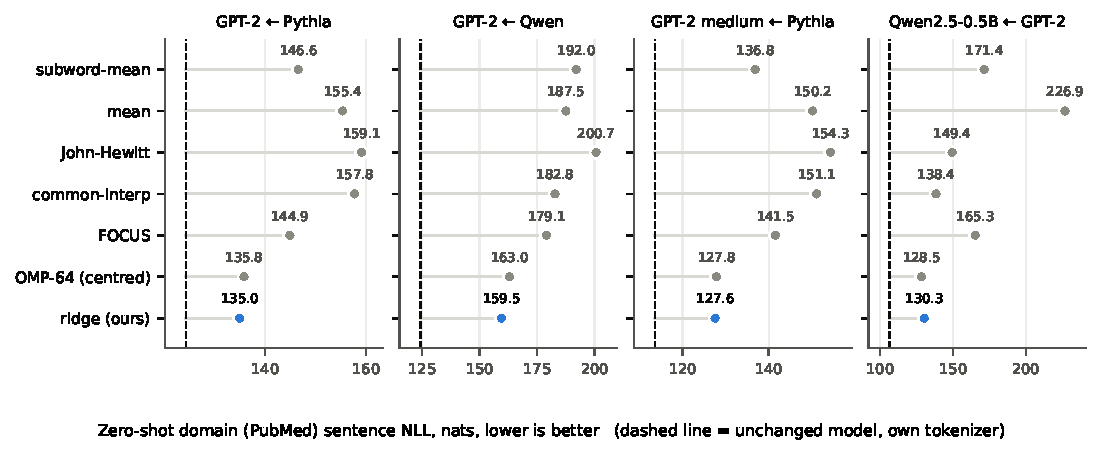
\includegraphics[width=0.95\textwidth]{figures/fig2_zero_shot_nll.pdf}
\caption{Domain (PubMed) NLL by method for each pair. OMP-64 as shipped (3.7k--7.7k nats on GPT-2 receivers) is omitted from the plot and listed in Table~\ref{tab:zs}. The dashed line is the unchanged model with its own tokenizer.}
\label{fig:zs}
\end{figure}
On the three GPT-2-receiver pairs, calibrated ridge has the lowest NLL of all methods on both text types. It is 10 to 20 nats below FOCUS and 9 to 33 nats below the subword mean on domain text. Against OMP-64 with centred inputs the margins are small. The paired difference ridge minus centred OMP-64 is $-0.85$ nats (95\,\% CI $-1.27$ to $-0.42$) on GPT-2$\leftarrow$Pythia and $-3.53$ ($-4.08$ to $-3.01$) on GPT-2$\leftarrow$Qwen2.5 on domain text, $-0.30$ ($-0.75$ to $+0.21$) on GPT-2 medium$\leftarrow$Pythia, and $+1.82$ ($+1.32$ to $+2.34$) on Qwen2.5$\leftarrow$GPT-2, where centred OMP-64 is significantly better. On general text the differences are $-0.33$, $-1.60$ and $-0.24$ (all significant) for the GPT-2 receivers and $+0.14$ ($-0.25$ to $+0.52$) for Qwen2.5. OMP-64 as shipped is catastrophic on the GPT-2 receivers (3.4k to 7.7k nats) and merely worse on Qwen2.5 ($129.8$ vs.\ $128.5$ nats); the uncalibrated ridge length is 0.1 to 2.2 nats worse than the calibrated one (Table~\ref{tab:zs}). Centring is therefore the difference between a working and a failing OMP on GPT-2 receivers, and we use the centred version as the strongest baseline throughout.

\subsection{Real vocabulary expansion}
\label{sec:realvocab}
Table~\ref{tab:rv} summarises the 16 runs and Fig.~\ref{fig:rv} shows each run against centred OMP-64; the full per-run table is in \ref{app:rv}.
\begin{table}[t]
\centering\small
\caption{Real vocabulary expansion, 16 runs (PubMed seeds 0--2 and arXiv seed 0, four receiver--donor pairs). Difference in sentence NLL (nats) of ridge minus each method; negative = ridge better. Median and range over runs; CI$<0$ = number of runs whose 95\,\% bootstrap interval lies below 0. ``Calibrated length'' uses the same length rule as ridge, isolating the direction. The last two rows compare ridge with the unchanged receiver (word left split). WECHSEL is reported separately in Table~\ref{tab:wech}.}
\label{tab:rv}
\resizebox{\textwidth}{!}{\begin{tabular}{lrrrrrr}
\toprule
 & \multicolumn{3}{c}{Zero-shot} & \multicolumn{3}{c}{After 200 steps} \\
\cmidrule(lr){2-4}\cmidrule(lr){5-7}
Ridge minus & Median & Range & CI$<0$ & Median & Range & CI$<0$ \\
\midrule
OMP-64, centred inputs (official) & $-$1.74 & $-$3.33 to $-$1.11 & 16/16 & $-$0.50 & $-$0.86 to $-$0.13 & 16/16 \\
OMP-64, centred, calibrated length & $-$1.18 & $-$1.50 to $-$0.79 & 16/16 & $-$0.57 & $-$0.82 to $-$0.30 & 16/16 \\
OMP-64, as shipped (official) & $-$238 & $-$3306 to $-$0.91 & 16/16 & $-$0.67 & $-$86.6 to $-$0.36 & 16/16 \\
OMP-32, centred (our scikit-learn) & $-$1.03 & $-$1.27 to $-$0.12 & 13/16 & $-$0.44 & $-$0.68 to $-$0.05 & 15/16 \\
Mean of word pieces (calibrated) & $-$6.51 & $-$8.90 to $-$4.79 & 16/16 & $-$2.18 & $-$3.21 to $-$0.94 & 16/16 \\
\midrule
\multicolumn{7}{l}{Zero-shot, ridge vs.\ unchanged receiver: better in 4, level in 3, worse in 9 of 16 runs} \\
\multicolumn{7}{l}{After 200 steps, ridge vs.\ unchanged receiver: better in 13, level in 3, worse in 0 of 16 runs} \\
\bottomrule
\end{tabular}
}
\end{table}
\begin{figure}[t]
\centering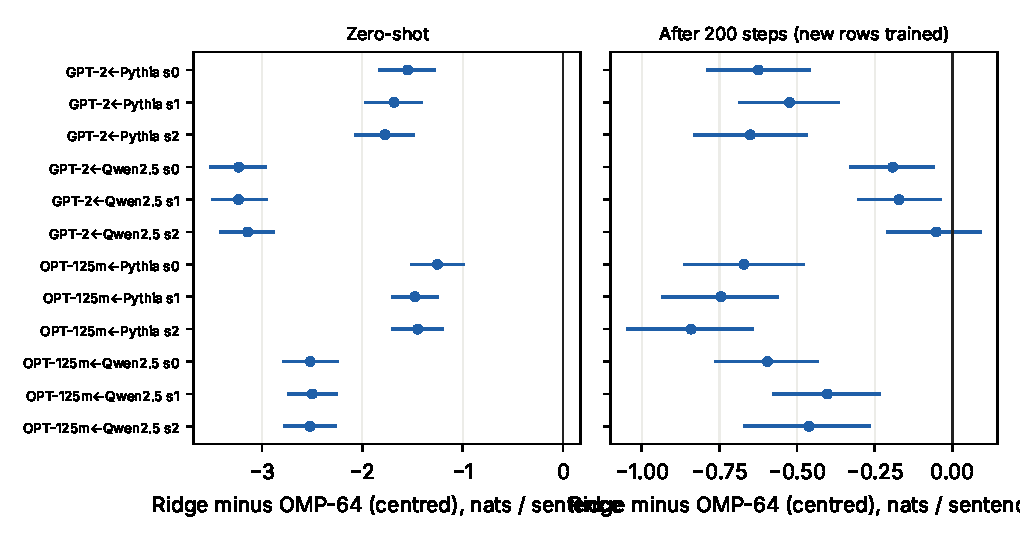
\includegraphics[width=0.85\textwidth]{figures/fig_realvocab.pdf}
\caption{Ridge minus official OMP-64 with centred inputs for each run (point: difference in NLL per sentence, bar: 95\,\% bootstrap interval; negative = ridge better).}
\label{fig:rv}
\end{figure}
Ridge has a lower NLL than centred OMP-64 in all 32 comparisons, with the interval excluding 0 each time, and all 32 remain significant after Holm correction (also for the calibrated-length version of OMP-64); the margin is 1.1 to 3.3 nats zero-shot and 0.1 to 0.9 after training the new rows. Even when OMP is given the same calibrated length as ridge, ridge is better in all 32 comparisons (0.3 to 1.5 nats), so the advantage is not only a matter of length: it lies in the direction. Ridge is also better than our sparse OMP-32 in all 32 (interval below 0 in 28) and than the mean of word pieces in all 32. The 32 comparisons come from 16 runs that share words and abstracts, so they are not 32 independent tests: the number of independent units is closer to eight (four pairs, two text domains) than to 32. The mean difference is negative in all four pairs, zero-shot and after training. OMP-64 as shipped is far worse on GPT-2 receivers with the Pythia donor ($-3306$ to $-2784$ nats zero-shot for the ridge difference) and with the Qwen donor ($-1078$ to $-473$).

Against the unchanged receiver, ridge is not uniformly better. Zero-shot, it is better in the four arXiv runs, not significantly different in three runs (OPT-125m$\leftarrow$Qwen2.5, PubMed) and worse in nine (PubMed with a GPT-2 receiver, $+0.4$ to $+2.3$ nats, and OPT-125m$\leftarrow$Pythia, $+0.5$ to $+0.7$). After 200 steps in which only the new rows are trained, ridge is better than the unchanged receiver in 13 runs and not significantly different in 3 (GPT-2$\leftarrow$Pythia, PubMed), never worse. Zero-shot expansion by any of the methods we tested therefore does not beat leaving the word split on PubMed text for GPT-2; what ridge provides is the best of the tested initialisations and a good start for training the rows.

\paragraph{Official WECHSEL} Table~\ref{tab:wech} compares ridge with the official WECHSEL package on the four PubMed seed-1 runs. Ridge has a lower NLL than WECHSEL in all 8 comparisons (4 pairs, zero-shot and after 200 steps), with every interval below 0: by 3.2 to 4.6 nats zero-shot against WECHSEL's raw output and by 2.0 to 2.9 nats against WECHSEL with the calibrated length, and by 0.5 to 1.7 nats after training the new rows. Zero-shot, WECHSEL is worse than the unchanged receiver in all four runs ($+2.1$ to $+5.0$ nats). The result covers one seed and one text domain, and WECHSEL was designed for cross-lingual transfer with an aligned static embedding space, so this is a same-language use of it that we chose for comparability, not its intended setting.
\begin{table}[t]
\centering\small
\caption{Official WECHSEL against ridge, PubMed seed 1 (NLL per sentence in nats; negative in the first two columns = ridge better). Intervals are 95\,\% paired bootstrap; $^{*}$ excludes 0.}
\label{tab:wech}
\resizebox{\textwidth}{!}{\begin{tabular}{llcccc}
\toprule
 & & \multicolumn{2}{c}{Ridge minus WECHSEL} & WECHSEL minus & Ridge minus\\
Pair & Steps & raw length & calibrated length & unchanged receiver & unchanged receiver\\
\midrule
GPT-2 $\leftarrow$ Pythia-160m & 0 & $-$3.82\,[$-$4.26,$-$3.40]$^{*}$ & $-$2.90\,[$-$3.33,$-$2.50]$^{*}$ & $+$4.96\,[$+$4.40,$+$5.56]$^{*}$ & $+$2.06\,[$+$1.63,$+$2.52]$^{*}$\\
 & 200 & $-$1.37\,[$-$1.61,$-$1.14]$^{*}$ & $-$1.45\,[$-$1.69,$-$1.20]$^{*}$ & $+$1.79\,[$+$1.35,$+$2.22]$^{*}$ & $+$0.34\,[$-$0.05,$+$0.74]\\
\addlinespace
GPT-2 $\leftarrow$ Qwen2.5-0.5B & 0 & $-$4.61\,[$-$4.93,$-$4.33]$^{*}$ & $-$2.69\,[$-$3.03,$-$2.36]$^{*}$ & $+$3.07\,[$+$2.70,$+$3.45]$^{*}$ & $+$0.38\,[$+$0.11,$+$0.64]$^{*}$\\
 & 200 & $-$0.48\,[$-$0.63,$-$0.32]$^{*}$ & $-$0.88\,[$-$1.05,$-$0.71]$^{*}$ & $-$0.67\,[$-$0.97,$-$0.38]$^{*}$ & $-$1.55\,[$-$1.82,$-$1.31]$^{*}$\\
\addlinespace
OPT-125m $\leftarrow$ Pythia-160m & 0 & $-$3.19\,[$-$3.60,$-$2.79]$^{*}$ & $-$2.03\,[$-$2.43,$-$1.65]$^{*}$ & $+$2.76\,[$+$2.23,$+$3.33]$^{*}$ & $+$0.73\,[$+$0.32,$+$1.15]$^{*}$\\
 & 200 & $-$1.72\,[$-$2.00,$-$1.45]$^{*}$ & $-$0.72\,[$-$0.95,$-$0.49]$^{*}$ & $-$0.41\,[$-$0.87,$+$0.05] & $-$1.13\,[$-$1.58,$-$0.68]$^{*}$\\
\addlinespace
OPT-125m $\leftarrow$ Qwen2.5-0.5B & 0 & $-$3.84\,[$-$4.16,$-$3.53]$^{*}$ & $-$2.28\,[$-$2.60,$-$1.96]$^{*}$ & $+$2.08\,[$+$1.72,$+$2.42]$^{*}$ & $-$0.20\,[$-$0.46,$+$0.04]\\
 & 200 & $-$0.89\,[$-$1.09,$-$0.69]$^{*}$ & $-$0.46\,[$-$0.60,$-$0.31]$^{*}$ & $-$2.58\,[$-$2.98,$-$2.20]$^{*}$ & $-$3.04\,[$-$3.42,$-$2.67]$^{*}$\\
\bottomrule
\end{tabular}
}
\end{table}

\subsection{Further baselines and larger receivers}
\label{sec:scale}
Table~\ref{tab:scale} compares ridge with six baselines on seven PubMed seed-1 pairs: the four small pairs, GPT-2 large, an untied Pythia-1B and Qwen2.5-1.5B (protocol in Section~\ref{par:large}). Each baseline gives 14 comparisons (seven pairs, zero-shot and after 200 steps). LS, Procrustes and SALT-ours are our adaptations; OMP-64 and WECHSEL are the official implementations.
\begin{table}[t]
\centering\scriptsize
\caption{Ridge minus each baseline, mean NLL difference per sentence in nats (negative = ridge better); $^{*}$ = 95\,\% paired bootstrap interval excludes 0. OMP-64c cal.\ = official OMP-64 on centred inputs with the same calibrated length as ridge; OMP-64s = OMP-64 as shipped; LS, Procrustes and SALT-ours are our adaptations (calibrated length); WECHSEL = official, calibrated length. Unch.\ = ridge minus the unchanged receiver (word left split; positive = ridge worse). Ridge is the variant chosen by the training objective. Intervals are in Tables~\ref{tab:scaleci1} and \ref{tab:scaleci2}, bits per byte in Table~\ref{tab:bpb}.}
\label{tab:scale}
\resizebox{\textwidth}{!}{\begin{tabular}{llrrrrrrr}
\toprule
Pair & Steps & OMP-64c cal. & OMP-64s & LS & Procrustes & SALT-ours & WECHSEL & Unch. \\
\midrule
GPT-2 $\leftarrow$ Pythia-160m & 0 & $-$1.11$^{*}$ & $-$3306.39$^{*}$ & $-$0.19$^{*}$ & $-$50.83$^{*}$ & $-$0.56$^{*}$ & $-$2.90$^{*}$ & $+$2.06$^{*}$ \\
 & 200 & $-$0.49$^{*}$ & $-$86.56$^{*}$ & $-$0.13$^{*}$ & $-$3.30$^{*}$ & $-$0.52$^{*}$ & $-$1.45$^{*}$ & $+$0.34 \\
\addlinespace
GPT-2 $\leftarrow$ Qwen2.5-0.5B & 0 & $-$1.14$^{*}$ & $-$472.82$^{*}$ & $-$0.44$^{*}$ & $-$167.66$^{*}$ & $-$1.11$^{*}$ & $-$2.69$^{*}$ & $+$0.38$^{*}$ \\
 & 200 & $-$0.50$^{*}$ & $-$0.55$^{*}$ & $-$0.55$^{*}$ & $-$0.94$^{*}$ & $-$0.45$^{*}$ & $-$0.88$^{*}$ & $-$1.55$^{*}$ \\
\addlinespace
OPT-125m $\leftarrow$ Pythia-160m & 0 & $-$1.10$^{*}$ & $-$1.17$^{*}$ & $-$0.04$^{*}$ & $+$0.59$^{*}$ & $-$0.95$^{*}$ & $-$2.03$^{*}$ & $+$0.73$^{*}$ \\
 & 200 & $-$0.62$^{*}$ & $-$0.79$^{*}$ & $-$0.07$^{*}$ & $-$0.19$^{*}$ & $-$0.69$^{*}$ & $-$0.71$^{*}$ & $-$1.13$^{*}$ \\
\addlinespace
OPT-125m $\leftarrow$ Qwen2.5-0.5B & 0 & $-$1.15$^{*}$ & $-$2.54$^{*}$ & $-$0.30$^{*}$ & $-$2.02$^{*}$ & $-$0.94$^{*}$ & $-$2.28$^{*}$ & $-$0.20 \\
 & 200 & $-$0.45$^{*}$ & $-$0.55$^{*}$ & $-$0.31$^{*}$ & $-$0.55$^{*}$ & $-$0.40$^{*}$ & $-$0.45$^{*}$ & $-$3.04$^{*}$ \\
\addlinespace
GPT-2 large $\leftarrow$ Qwen2.5-0.5B & 0 & $-$1.58$^{*}$ & $-$3.37$^{*}$ & $-$0.22$^{*}$ & $-$1.53$^{*}$ & $-$1.70$^{*}$ & $-$3.66$^{*}$ & $+$1.11$^{*}$ \\
 & 200 & $-$0.28$^{*}$ & $-$0.32$^{*}$ & $-$0.19$^{*}$ & $-$0.39$^{*}$ & $-$0.33$^{*}$ & $-$0.86$^{*}$ & $-$0.47$^{*}$ \\
\addlinespace
Pythia-1B (untied) $\leftarrow$ Qwen2.5-0.5B & 0 & $-$0.03 & $-$1.63$^{*}$ & $-$1.23$^{*}$ & $-$0.07 & $+$0.27 & $-$3.32$^{*}$ & $+$2.55$^{*}$ \\
 & 200 & $-$0.27 & $-$0.03 & $-$0.36 & $-$0.51 & $+$1.06$^{*}$ & $-$0.03 & $+$2.70$^{*}$ \\
\addlinespace
Qwen2.5-1.5B $\leftarrow$ Pythia-410m & 0 & $-$0.26 & $-$3.02$^{*}$ & $-$0.75$^{*}$ & $+$0.19 & $-$1.93$^{*}$ & $-$4.23$^{*}$ & $+$6.62$^{*}$ \\
 & 200 & $-$0.54$^{*}$ & $-$0.64$^{*}$ & $-$0.02 & $-$0.61$^{*}$ & $-$1.44$^{*}$ & $-$1.64$^{*}$ & $+$7.43$^{*}$ \\
\bottomrule
\end{tabular}
}
\end{table}
By the 95\,\% interval, ridge is better than centred OMP-64 with the same calibrated length in 11 of 14 comparisons (by 1.1 to 1.6 nats zero-shot and 0.3 to 0.6 after training) and not significantly different in 3, all on the two largest receivers. It is better than OMP-64 as shipped in 13 (not significantly different in 1), than WECHSEL with calibrated length in 13 (1), than LS in 12 (2), than SALT-ours with calibrated length in 12 (1 not significantly different, 1 worse), than Procrustes in 10 (3 not significantly different, 1 worse) and than our OMP-32 in 10 (3 not significantly different, 1 worse; OMP-32 is not in the table). These are 98 comparisons (seven baselines, 14 each), and we correct for them with Holm's procedure (Section~\ref{sec:stats}): 74 of the 81 significant wins of ridge survive, and the 7 that do not are small (0.19 to 0.64 nats). Of the three comparisons in which a baseline is significantly better, two survive the correction: Procrustes on OPT-125m$\leftarrow$Pythia-160m zero-shot (ridge $+0.59$ nats) and OMP-32 on Qwen2.5-1.5B zero-shot (ridge $+0.58$ nats, 95\,\% CI $+0.27$ to $+0.89$; after training ridge is better by 1.11). The third, SALT-ours with calibrated length on Pythia-1B after training (ridge $+1.06$, CI $+0.17$ to $+2.00$, uncorrected $p\approx0.02$), does not. For that one, 0.95 of the 1.06 nats lie on the tokens of the sentence that are not new words, ridge was not worse zero-shot ($+0.27$, interval including 0), the other comparisons with SALT-ours on that receiver are not significant, and the pair is a single run with 129 test sentences that we did not replicate, so we read it as a nominal advantage for SALT-ours, not as a result. ``Not significantly different'' is not equivalence: with a margin of $\pm0.5$ nats and 90\,\% intervals (two one-sided tests), only 4 of the 14 non-significant comparisons are equivalent, and 9 of the 10 inconclusive ones are on Pythia-1B, whose 129 test sentences give intervals about $\pm1$ nat wide. LS is not significantly different from ridge after training on Qwen2.5-1.5B ($-0.02$, equivalent within the margin), as expected with more than 24\,000 anchors (Section~\ref{sec:scarce}).

Against the unchanged receiver, ridge is worse in 8 of 14 comparisons, not significantly different in 2 and better in 4 (GPT-2$\leftarrow$Qwen2.5, both OPT-125m pairs and GPT-2 large, all after training; GPT-2 large is $+1.11$ nats zero-shot and $-0.47$ after training). For the two receivers of 1B parameters or more, \emph{every} method we tested, ridge included, is worse than leaving the words split, both zero-shot and after 200 steps: ridge is $+2.55$ and $+2.70$ nats on Pythia-1B and $+6.62$ and $+7.43$ on Qwen2.5-1.5B (on the new words alone still $+4.06$ and $+4.26$ on Qwen2.5-1.5B). We did not test longer training or other settings, so this is a statement about 200 steps on the new rows, not about expansion in general. On the untied Pythia-1B, the advantage over centred OMP-64 seen with small receivers is absent ($-0.03$ zero-shot, interval $-0.96$ to $+0.94$), while least squares is clearly worse zero-shot ($-1.23$ for the difference).

\subsection{Downstream classification}
\label{sec:downstream}
\begin{table}[t]
\centering\small
\caption{PubMed-RCT test accuracy after fine-tuning the transplanted GPT-2 for 3 epochs (mean $\pm$ sd over seeds).}
\label{tab:ft}
\resizebox{\textwidth}{!}{\begin{tabular}{llrrr}
\toprule
Pair & Method & Seeds & Accuracy (mean $\pm$ sd) & Macro-F1 \\
\midrule
GPT-2 $\leftarrow$ Qwen & \textbf{Ridge, calibrated (ours)} & 3 & 0.7883 $\pm$ 0.0042 & 0.713 \\
GPT-2 $\leftarrow$ Qwen & FOCUS & 3 & 0.7878 $\pm$ 0.0003 & 0.711 \\
GPT-2 $\leftarrow$ Qwen & OMP-64, as shipped & 3 & 0.7882 $\pm$ 0.0021 & 0.714 \\
GPT-2 $\leftarrow$ Qwen & OMP-64, centred inputs & 3 & 0.7862 $\pm$ 0.0025 & 0.712 \\
GPT-2 $\leftarrow$ Qwen & Subword mean & 3 & 0.7875 $\pm$ 0.0040 & 0.711 \\
GPT-2 $\leftarrow$ Qwen & Mean fill & 3 & 0.7837 $\pm$ 0.0008 & 0.707 \\
GPT-2 $\leftarrow$ Qwen & Native tokenizer (reference) & 3 & 0.7900 $\pm$ 0.0030 & 0.717 \\
\midrule
GPT-2 $\leftarrow$ Pythia & \textbf{Ridge, calibrated (ours)} & 5 & 0.7917 $\pm$ 0.0015 & 0.719 \\
GPT-2 $\leftarrow$ Pythia & FOCUS & 4 & 0.7915 $\pm$ 0.0023 & 0.719 \\
GPT-2 $\leftarrow$ Pythia & OMP-64, as shipped & 4 & 0.7899 $\pm$ 0.0019 & 0.716 \\
GPT-2 $\leftarrow$ Pythia & OMP-64, centred inputs & 5 & 0.7889 $\pm$ 0.0028 & 0.715 \\
GPT-2 $\leftarrow$ Pythia & Subword mean & 5 & 0.7914 $\pm$ 0.0027 & 0.718 \\
GPT-2 $\leftarrow$ Pythia & Mean fill & 5 & 0.7887 $\pm$ 0.0020 & 0.715 \\
GPT-2 $\leftarrow$ Pythia & Native tokenizer (reference) & 5 & 0.7902 $\pm$ 0.0030 & 0.718 \\
\bottomrule
\end{tabular}
}
\end{table}
\paragraph{Fine-tuning} All methods end within about 0.6 points of the native tokenizer and of each other (Table~\ref{tab:ft}, Fig.~\ref{fig:ft}). Ridge minus FOCUS is $+0.05$ points (95\,\% CI $-0.47$ to $+0.57$) on GPT-2$\leftarrow$Qwen2.5 and $+0.03$ ($-0.36$ to $+0.41$) on GPT-2$\leftarrow$Pythia; ridge minus centred OMP-64 is $+0.22$ ($-0.20$ to $+0.62$) and $+0.28$ ($-0.02$ to $+0.58$); ridge minus the subword mean is $+0.08$ ($-0.45$ to $+0.63$) and $+0.03$ ($-0.31$ to $+0.38$). No difference is significant.
\begin{figure}[t]
\centering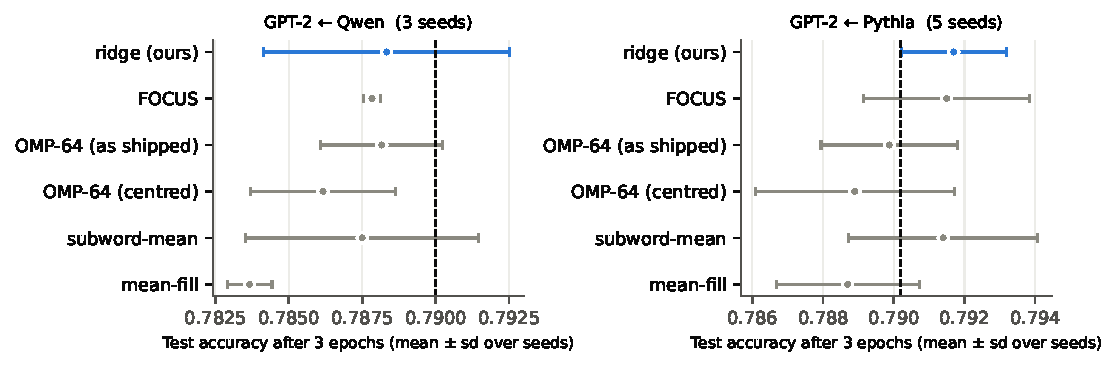
\includegraphics[width=0.95\textwidth]{figures/fig3_finetuned_accuracy.pdf}
\caption{Fine-tuned accuracy by method (mean $\pm$ sd over seeds); the dashed line is the native tokenizer.}
\label{fig:ft}
\end{figure}

\paragraph{Frozen probe} Fine-tuning can repair poor embeddings, so we also read out frozen features (Table~\ref{tab:holm}, Fig.~\ref{fig:probe}; accuracies in \ref{app:probe}). Of the 54 paired tests, 11 are significant before correction and 4 after Holm correction, all against mean fill (ridge better by $+1.4$ points on GPT-2$\leftarrow$Qwen2.5 at the middle and last layers, by $+8.3$ and $+6.7$ points on Qwen2.5$\leftarrow$GPT-2). Ridge is not significantly different from OMP-64 (centred or as shipped), FOCUS and the subword mean once corrected. The one uncorrected loss against OMP-64 centred (Qwen2.5$\leftarrow$GPT-2, last layer, $-0.65$ points, CI $-1.28$ to $-0.04$) does not survive the correction.
\begin{table}[t]
\centering\small
\caption{Frozen probe: ridge minus each method, accuracy in points (positive = ridge better). $^{*}$ 95\,\% CI excludes 0 before correction; $^{\dagger}$ still significant after Holm correction over all 54 tests.}
\label{tab:holm}
\resizebox{\textwidth}{!}{\begin{tabular}{llrrrrrr}
\toprule
Pair & Layer & OMP-64 centred & OMP-64 shipped & FOCUS & Subw.\ mean & Mean fill & Native tok. \\
\midrule
GPT-2$\leftarrow$Pythia & emb & $-$0.30 & $-$0.10 & $+$0.25 & $+$0.36 & $-$0.03 & $+$0.64 \\
 & mid & $-$0.01 & $-$0.05 & $+$0.05 & $+$0.24 & $+$0.40 & $+$0.19 \\
 & last & $-$0.24 & $-$0.06 & $+$0.58 & $+$0.22 & $+$0.26 & $+$0.11 \\
\midrule
GPT-2$\leftarrow$Qwen2.5 & emb & $+$0.32 & $+$0.21 & $-$0.25 & $-$0.04 & $+$0.21 & $+$0.68 \\
 & mid & $+$0.32 & $+$0.31 & $+$0.95$^{*}$ & $+$0.86$^{*}$ & $+$1.37$^{\dagger}$ & $+$0.09 \\
 & last & $+$0.44 & $+$0.10 & $+$0.92$^{*}$ & $+$0.83$^{*}$ & $+$1.42$^{\dagger}$ & $+$0.71 \\
\midrule
Qwen2.5$\leftarrow$GPT-2 & emb & $+$0.12 & $-$0.22 & $-$0.62$^{*}$ & $-$0.14 & $+$0.05 & $-$0.60 \\
 & mid & $-$0.16 & $-$0.34 & $+$0.75$^{*}$ & $+$0.64 & $+$8.26$^{\dagger}$ & $-$0.19 \\
 & last & $-$0.65$^{*}$ & $-$0.41 & $+$0.15 & $-$0.15 & $+$6.69$^{\dagger}$ & $-$0.61 \\
\bottomrule
\end{tabular}
}
\end{table}
\begin{figure}[t]
\centering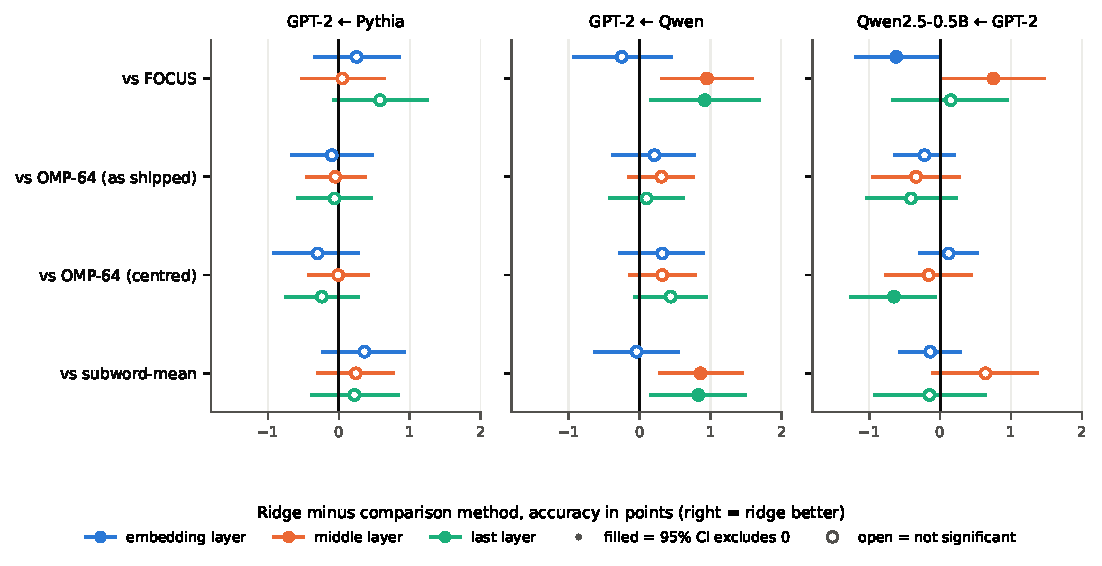
\includegraphics[width=0.95\textwidth]{figures/fig4_frozen_probe_forest.pdf}
\caption{Frozen probe: ridge minus comparison method (points; bars 95\,\% CI, uncorrected). Filled markers: interval excludes 0.}
\label{fig:probe}
\end{figure}

\subsection{Ablation}
\label{sec:ablation}
We removed one component at a time and measured sentence NLL on PubMed with the GPT-2 receiver (300 and 82 new words, seed 1). Differences are against ridge fitted on all anchors (Table~\ref{tab:abl}).
\begin{table}[t]
\centering\small
\caption{Ablations (nats per sentence; positive = the ablation is worse than ridge on all anchors). $^{*}$ 95\,\% interval excludes 0. First row: full ridge against the unchanged receiver.}
\label{tab:abl}
\resizebox{\textwidth}{!}{\begin{tabular}{lrrrr}
\toprule
 & \multicolumn{2}{c}{GPT-2$\leftarrow$Pythia} & \multicolumn{2}{c}{GPT-2$\leftarrow$Qwen2.5} \\
\cmidrule(lr){2-3}\cmidrule(lr){4-5}
Variant (change from ridge fitted on all anchors) & Zero-shot & 200 steps & Zero-shot & 200 steps \\
\midrule
Full ridge vs.\ unchanged receiver (reference) & $+$2.21$^{*}$ & $+$0.49$^{*}$ & $+$0.83$^{*}$ & $-$1.00$^{*}$ \\
\midrule
Ridge on the 5000 most frequent anchors & $-$0.15$^{*}$ & $-$0.15$^{*}$ & $-$0.46$^{*}$ & $-$0.55$^{*}$ \\
No centring, calibrated length & $+$549$^{*}$ & $+$2.16$^{*}$ & $+$10.08$^{*}$ & $-$0.16 \\
No centring, raw output & $+$1678$^{*}$ & $+$2.04$^{*}$ & $+$208$^{*}$ & $-$0.63$^{*}$ \\
Own magnitude (no unit direction, no calibration) & $+$2.65$^{*}$ & $+$0.16$^{*}$ & $+$3.09$^{*}$ & $-$0.60$^{*}$ \\
Unit direction, fixed length 1.0 & $+$0.55$^{*}$ & $+$0.13$^{*}$ & $+$0.60$^{*}$ & $-$0.35$^{*}$ \\
$\lambda=10^{-4}$ & $+$0.05$^{*}$ & $-$0.02$^{*}$ & $-$0.01$^{*}$ & $+$0.00 \\
$\lambda=10^{-3}$ & $+$0.05$^{*}$ & $-$0.02$^{*}$ & $+$0.00 & $+$0.00 \\
$\lambda=10^{-2}$ & $+$0.04$^{*}$ & $-$0.01$^{*}$ & $+$0.06$^{*}$ & $-$0.00 \\
$\lambda=0.1$ & $+$0.00 & $+$0.00 & $+$0.17$^{*}$ & $-$0.01 \\
$\lambda=1$ & $+$0.24$^{*}$ & $+$0.07$^{*}$ & $+$1.79$^{*}$ & $-$0.34$^{*}$ \\
Mean of word pieces (calibrated) & $+$8.76$^{*}$ & $+$2.87$^{*}$ & $+$4.78$^{*}$ & $+$0.47$^{*}$ \\
\bottomrule
\end{tabular}
}
\end{table}
\textbf{Centring} is essential zero-shot: without it the NLL rises by 549 nats with Pythia and 10 with Qwen2.5; after training the new rows the loss is 2.2 nats with Pythia, and with Qwen2.5 the uncentred variants are level or slightly better. \textbf{Length calibration} helps zero-shot (no scale at all: $+2.7$ to $+3.1$ nats; a fixed length of 1: $+0.6$), but after training the uncalibrated variants are 0.35 to 0.6 nats better with Qwen2.5 and 0.13 to 0.16 worse with Pythia, so its benefit is a zero-shot benefit. \textbf{The regularisation strength} is not critical: between $10^{-4}$ and $10^{-2}$ the NLL changes by at most 0.06 nats ($\lambda=0.1$ costs 0.17 with Qwen2.5, $\lambda=1$ is clearly too large zero-shot). \textbf{The ridge direction} is far better than the mean of word pieces ($+8.8$ and $+4.8$ nats zero-shot). Fitting on the 5000 most frequent anchors is better than on all anchors ($-0.15$ and $-0.46$ zero-shot), which supports selecting by the training objective. These ablations use one seed, one text domain and two pairs.

\subsection{Scarce anchors: why regularise}
\label{sec:scarce}
With tens of thousands of anchors, a well-conditioned least-squares fit needs little regularisation. It should matter when the number of anchors $n$ is small or close to the embedding dimension $d$, where the least-squares problem is ill-conditioned (for $n<d$ it is underdetermined, and we use the minimum-norm solution). We tested this on the two GPT-2 pairs of the real vocabulary setting (PubMed, seed 1, zero-shot) by fitting both maps on $n=d/2$, $d$ and $2d$ anchors drawn uniformly at random without replacement from all whole-word anchors (five independent random subsets per $n$, not frequency-selected) and on all anchors, with the same calibrated length for both. Fig.~\ref{fig:cos} shows the held-out cosine between predicted and true receiver rows, measured on 2000 anchors not used for fitting and averaged over five random subsets per $n$, for $n/d$ from 0.1 to about 30; Table~\ref{tab:anchors} gives the NLL.
\begin{figure}[t]
\centering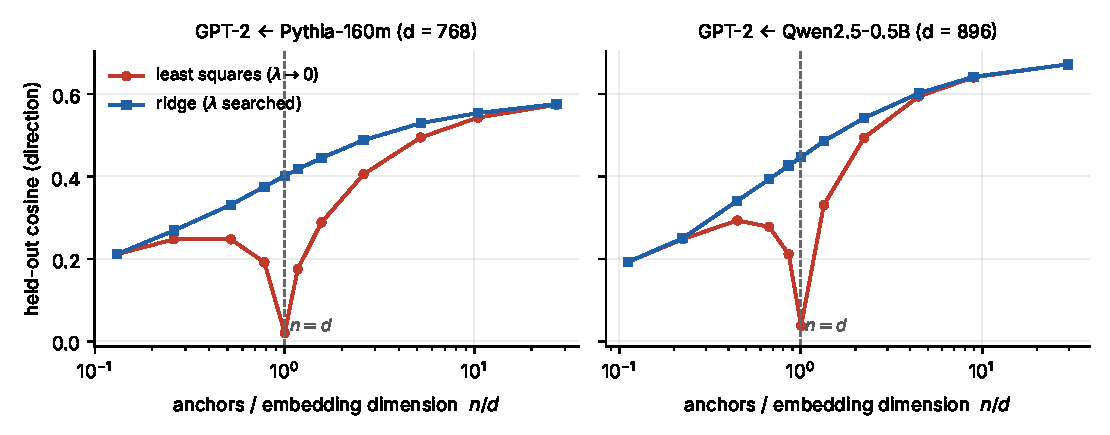
\includegraphics[width=0.97\textwidth]{figures/fig_ls_vs_ridge_cosine.pdf}
\caption{Held-out cosine between predicted and true receiver embeddings against the number of anchors relative to the donor dimension, for plain least squares (minimum-norm solution) and ridge ($\lambda$ searched on held-out anchors). The dashed line marks $n=d$.}
\label{fig:cos}
\end{figure}
\begin{table}[t]
\centering\small
\caption{Plain least squares (LS) against ridge when only $n$ anchors are used to fit the map (PubMed, seed 1, zero-shot; NLL in nats per sentence; mean over five random anchor subsets per $n$, one for all anchors). The difference column gives the mean and the minimum and maximum over the subsets. Both maps use the same calibrated length. The unchanged receiver has an NLL of 142.3 (Pythia donor) and 147.3 (Qwen donor).}
\label{tab:anchors}
\resizebox{\textwidth}{!}{\begin{tabular}{llrrr}
\toprule
Pair & $n$ ($n/d$) & LS & Ridge & Ridge $-$ LS: mean [min, max over subsets] \\
\midrule
GPT-2$\leftarrow$Pythia-160m & 384 (0.5) & 203.6 & 147.6 & $-$55.99 [$-$100.45, $-$12.92] \\
 & 768 (1.0) & 275.4 & 146.5 & $-$128.95 [$-$519.01, $-$13.93] \\
 & 1,536 (2.0) & 147.3 & 145.5 & $-$1.74 [$-$1.96, $-$1.63] \\
 & 22,781 (29.7) & 144.5 & 144.5 & $-$0.05 (one subset) \\
\midrule
GPT-2$\leftarrow$Qwen2.5-0.5B & 448 (0.5) & 358.1 & 153.5 & $-$204.57 [$-$733.99, $-$7.73] \\
 & 896 (1.0) & 249.9 & 152.9 & $-$97.02 [$-$180.47, $-$18.94] \\
 & 1,792 (2.0) & 149.9 & 150.7 & $+$0.85 [$+$0.72, $+$1.12] \\
 & 28,512 (31.8) & 148.1 & 148.1 & $+$0.01 (one subset) \\
\bottomrule
\end{tabular}
}
\end{table}
Least squares collapses when $n$ is near $d$: its held-out cosine falls to 0.02 at $n=768$ (Pythia donor) and 0.04 at $n=900$ (Qwen donor), while ridge stays at about 0.40 and 0.45, and below $n=d$ least squares is already worse than ridge. The NLL shows the same pattern (Table~\ref{tab:anchors}). Ridge is better in every one of the five subsets at $n=d/2$ (by 13 to 100 nats with the Pythia donor and 8 to 734 with the Qwen donor) and at $n=d$ (by 14 to 519 and 19 to 180 nats); the size of the gap varies a lot between subsets, because the minimum-norm least-squares fit occasionally fails badly near $n=d$, so the means are dominated by those cases and the ranges should be read with them. At $n=2d$ the picture is mixed and consistent across subsets: ridge is 1.6 to 2.0 nats better in all five with the Pythia donor but 0.7 to 1.1 nats \emph{worse} in all five with the Qwen donor. With all anchors ($n/d\approx30$) the two do not differ significantly (differences of $-0.05$ and $+0.01$ nats). Regularisation therefore matters in the scarce-anchor regime, roughly $n\lesssim 2d$, and not when there are tens of thousands of anchors as in our main experiments. This regime arises when two tokenizers share few whole-word tokens, for example with a small donor vocabulary or a restricted anchor list; the pairs we tested do not have this property, so these are controlled subsamples, not a test on such pairs.

\paragraph{Choice of $\lambda$ in the scarce regime} $\lambda$ was chosen as in the main method, by cosine on held-out anchors (10\,\% of the anchors, at least 50, at most 20\,\%; about 50 anchors at $n=d/2$). It was the largest value of the grid ($\lambda=1$) in all five subsets at $n\le2d$ for both donors, which raises the question whether the grid is too narrow. We therefore repeated the selection with a grid extended to $\lambda=1000$. It then chose $\lambda=10$ at $n\le d$ for the Pythia donor and for $n=d/2$ with the Qwen donor, but the NLL did not improve: it was 0.03 to 0.5 nats higher with the Pythia donor and 2.6 nats higher at $n=d/2$ with the Qwen donor, and identical at the other sizes. The grid edge therefore does not limit the result: selecting $\lambda$ by cosine and measuring NLL agree on $\lambda\approx1$ to 10 here. The results rest on two pairs, one seed and five random subsets per $n$.

\subsection{Mapping time}
\label{sec:speed}
An earlier timing from our experiment logs compared OMP on a GPU with ridge on a CPU and is not used. We therefore timed both on the \emph{same device and dtype}: float32, the official \texttt{batch\_omp} and our torch implementation of Eq.~\eqref{eq:ridge}, GPT-2 and Pythia-160m or Qwen2.5-0.5B embedding matrices (42\,257 anchors), $K$ donor-only tokens, after a warm-up with device synchronisation, median of 5 repeats, on 2 CPU threads and one Tesla T4 GPU. ``Fixed'' uses one solve with $\lambda=0.01$, supported by the ablation; ``search'' is the procedure of Section~\ref{sec:method} (five validation solves and one final solve).
\begin{table}[t]
\centering\small
\caption{Time to build the new rows (seconds, median of 5, float32). Ratio = OMP-64 time divided by fixed-$\lambda$ ridge time. The length calibration is not included.}
\label{tab:speed}
\resizebox{\textwidth}{!}{\begin{tabular}{lrrrrrrrrr}
\toprule
 & & \multicolumn{4}{c}{CPU (2 threads), s} & \multicolumn{4}{c}{GPU (Tesla T4), s} \\
\cmidrule(lr){3-6}\cmidrule(lr){7-10}
Pair & $K$ & OMP-64 & Ridge fixed & Ridge search & Ratio & OMP-64 & Ridge fixed & Ridge search & Ratio \\
\midrule
GPT-2 $\leftarrow$ Pythia & 82 & 2.59 & 0.547 & 2.85 & 5$\times$ & 0.16 & 0.043 & 0.12 & 4$\times$ \\
 & 300 & 9.95 & 0.551 & 2.93 & 18$\times$ & 0.47 & 0.043 & 0.14 & 11$\times$ \\
 & 1000 & 30.28 & 0.572 & 2.93 & 53$\times$ & 1.58 & 0.043 & 0.14 & 37$\times$ \\
 & 3000 & 87.62 & 0.573 & 2.96 & 153$\times$ & 5.11 & 0.039 & 0.14 & 131$\times$ \\
\midrule
GPT-2 $\leftarrow$ Qwen2.5 & 82 & 3.71 & 0.757 & 4.00 & 5$\times$ & 0.24 & 0.058 & 0.21 & 4$\times$ \\
 & 300 & 12.66 & 0.766 & 4.01 & 17$\times$ & 0.68 & 0.037 & 0.21 & 18$\times$ \\
 & 1000 & 37.98 & 0.758 & 3.96 & 50$\times$ & 1.78 & 0.039 & 0.21 & 46$\times$ \\
 & 3000 & 109.74 & 0.784 & 4.08 & 140$\times$ & 5.61 & 0.039 & 0.21 & 144$\times$ \\
\bottomrule
\end{tabular}
}
\end{table}
\begin{figure}[t]
\centering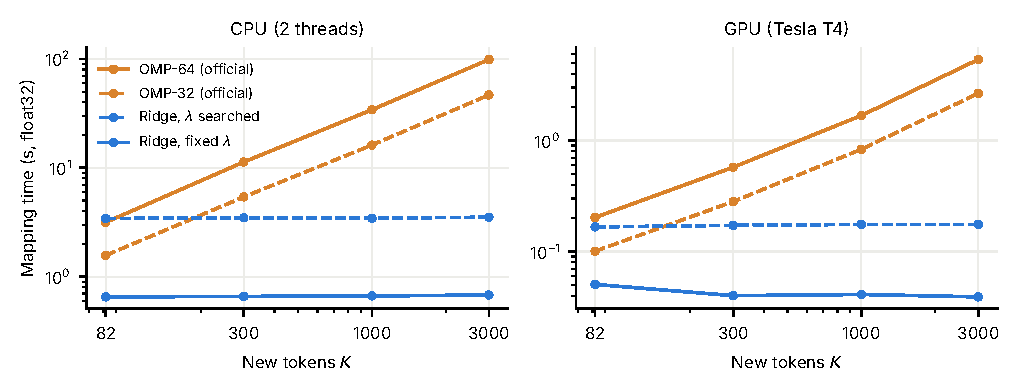
\includegraphics[width=0.95\textwidth]{figures/fig_speed.pdf}
\caption{Mapping time against the number of new tokens $K$ (mean of the two pairs, float32, log--log scale).}
\label{fig:speed}
\end{figure}
With a fixed $\lambda$, ridge is faster than official OMP-64 in every setting: 4 to 5 times at $K=82$, 11 to 18 times at 300, 37 to 53 times at 1000 and 131 to 153 times at 3000 (Table~\ref{tab:speed}). Ridge time is almost independent of $K$, whereas OMP grows linearly with it (about 29 to 45\,ms per token on the CPU and 1.6 to 3\,ms per token on the T4). With the $\lambda$ search, ridge is level with OMP at $K=82$ (0.9 to 1.3 times) and 3 to 3.5, 8.5 to 11 and 27 to 36 times faster at 300, 1000 and 3000. One caution applies: the speed advantage concerns the mapping step only. The reported NLL results use a float64 ridge, so we checked that the float32 solve used in the timing gives the same directions: for 3000 new tokens, the cosine between the float32 and float64 directions is at least 0.999999 for every token (minimum and mean both 1.000000 at six decimals) for GPT-2$\leftarrow$Pythia-160m (36\,938 anchors) and GPT-2$\leftarrow$Qwen2.5-0.5B (42\,257 anchors).

\section{Discussion}
\label{sec:discussion}
\paragraph{What the evidence supports} Ridge is a simple, fast, gradient-free initialiser that is slightly but consistently better than the strongest official baseline (centred OMP-64) in real vocabulary expansion with small receivers, better than, or not significantly different from, the other baselines we tested in nearly all comparisons up to 1.5B parameters, clearly better than FOCUS and simple baselines zero-shot, and no worse downstream. The ablations indicate why: the receiver and donor spaces share a large common component that must be removed before a linear map can be fitted, and a regression that sees all anchors at once gives better directions than a sparse reconstruction of 64 of them, even when both use the same length rule (Table~\ref{tab:rv}). The regularisation in ridge matters mainly when anchors are scarce: with $n\lesssim 2d$ anchors, plain least squares is much worse in NLL, and with tens of thousands of anchors the two are level (Section~\ref{sec:scarce}).

\paragraph{What it does not support} We do not claim state-of-the-art results, a downstream accuracy gain, or that expansion beats leaving words split: at 1B parameters and above it did not, for any method. Nor do we claim that ridge beats a local-regression baseline: on the untied Pythia-1B receiver SALT-ours with calibrated length is nominally better after training. The margins over centred OMP-64 are small, and on Qwen2.5$\leftarrow$GPT-2 domain text centred OMP-64 is better zero-shot. Efficiency is a property of the mapping step on a given device; the length calibration costs the same for every calibrated method.

\paragraph{Limitations} Downstream evidence is one classification task, and real vocabulary expansion is measured by NLL, not by a task. The receivers are small to medium (125M to 1.5B parameters). Only one receiver is untied (Pythia-1B), its output rows were built from the donor output embeddings, a design choice we did not vary, and the three larger receivers are single runs with one seed, one text domain and 40 to 300 words. arXiv has one seed. The seeds resample sentences and training batches, not words or abstracts, so they measure training and sampling noise. The ablations and the scarce-anchor test use one seed and one text domain. Multiplicity is corrected for the frozen probe, the 16-run comparison with OMP-64 and the 98 comparisons of Section~\ref{sec:scale}, not for the other tables. The bootstrap resamples sentences and ignores their grouping by abstract, so intervals are probably too narrow. Learned initialisers \cite{minixhofer2024zett,dobler2025tokendistillation,li2025tokalign} are not compared. SALT \cite{lee2025salt} is represented only by our simplified adaptation, and LS, Procrustes and OMP-32 are also our own implementations. WECHSEL was run on the PubMed seed-1 runs only, in same-language mode.

\section{Conclusion}
\label{sec:conclusion}
A closed-form ridge map from donor to receiver embeddings, fitted on centred anchors and scaled by a single calibrated length, is an effective way to initialise new tokens. In 16 real vocabulary expansion runs it was better than the official OMP-64 in every comparison, by small margins, and its mapping step is much cheaper than OMP as the number of new tokens grows. On seven pairs up to 1.5B parameters it was better than, or not significantly different from, the other baselines in nearly all comparisons, but for the two receivers of 1B parameters or more no initialisation, ridge included, beat leaving the words split. We also showed that the official OMP needs centred inputs on GPT-2 receivers, and that after fine-tuning or in a frozen probe the choice among good initialisers does not change accuracy. Larger models, more seeds and word samples at that scale, more downstream tasks and learned initialisers are the natural next comparisons.

\section*{Declaration of competing interest}
The authors declare that they have no known competing financial interests or personal relationships that could have appeared to influence the work reported in this paper.

\section*{CRediT authorship contribution statement}
\textbf{Shibdas Bhattacharya:} Conceptualization, Methodology, Software, Investigation, Formal analysis, Writing -- original draft. \textbf{Haider Banka:} Supervision, Writing -- review \& editing.

\section*{Funding}
This research did not receive any specific grant from funding agencies in the public, commercial, or not-for-profit sectors.

\section*{Data and code availability}
All data are public (PubMedQA, PubMed 20k RCT, WikiText-2, arXiv abstracts) and all models are public. The code, notebooks, result files, analysis scripts, a requirements file, a script that records the environment and a reproducibility guide are publicly available at \todo{repository URL and DOI}. The guide maps every table and figure to a notebook and a script. Appendix~\ref{app:repro} lists checkpoints, data, hyperparameters and seeds. The experiment notebooks install packages without version pins, and the versions of the reported runs were not recorded at the time; the repository records the environment afterwards and gives a rerun check.

\section*{Declaration of generative AI use in the writing process}
During the preparation of this work the authors used Claude (Anthropic) to help write and debug code for the experiments and statistical analysis, to generate tables and figures from the results, and to draft and edit the text. After using this tool, the authors reviewed and edited the content and take full responsibility for the content of the publication.

\appendix
\section{Real vocabulary expansion: all runs}
\label{app:rv}
\begin{table}[H]
\centering\scriptsize
\caption{Ridge minus each method, NLL per sentence in nats, for each of the 16 runs (negative = ridge better; $^{*}$ 95\,\% interval excludes 0). ``vs.\ unch.'' = ridge minus the unchanged receiver; OMP-64c = official OMP-64 on centred inputs; OMP-64s = as shipped; OMP-32 = our scikit-learn implementation.}
\label{tab:rvfull}
\resizebox{\textwidth}{!}{\begin{tabular}{llrrrrrrrrrr}
\toprule
 & & & & \multicolumn{4}{c}{Zero-shot} & \multicolumn{4}{c}{After 200 steps} \\
\cmidrule(lr){5-8}\cmidrule(lr){9-12}
Receiver$\leftarrow$donor & Text & Seed & Words & vs.\ unch. & $-$OMP-64c & $-$OMP-64s & $-$OMP-32 & vs.\ unch. & $-$OMP-64c & $-$OMP-64s & $-$OMP-32 \\
\midrule
GPT-2$\leftarrow$Pythia & PubMed & 0 & 300 & $+$1.89$^{*}$ & $-$1.59$^{*}$ & $-$3280$^{*}$ & $-$0.43$^{*}$ & $+$0.30 & $-$0.56$^{*}$ & $-$81.86$^{*}$ & $-$0.48$^{*}$ \\
GPT-2$\leftarrow$Qwen2.5 & PubMed & 0 & 82 & $+$0.47$^{*}$ & $-$3.20$^{*}$ & $-$482$^{*}$ & $-$1.07$^{*}$ & $-$1.57$^{*}$ & $-$0.23$^{*}$ & $-$0.67$^{*}$ & $-$0.52$^{*}$ \\
OPT-125m$\leftarrow$Pythia & PubMed & 0 & 300 & $+$0.60$^{*}$ & $-$1.40$^{*}$ & $-$1.08$^{*}$ & $-$0.23 & $-$1.12$^{*}$ & $-$0.86$^{*}$ & $-$0.67$^{*}$ & $-$0.30$^{*}$ \\
OPT-125m$\leftarrow$Qwen2.5 & PubMed & 0 & 82 & $+$0.08 & $-$2.42$^{*}$ & $-$2.41$^{*}$ & $-$1.04$^{*}$ & $-$2.77$^{*}$ & $-$0.48$^{*}$ & $-$0.54$^{*}$ & $-$0.38$^{*}$ \\
GPT-2$\leftarrow$Pythia & PubMed & 1 & 300 & $+$2.06$^{*}$ & $-$1.45$^{*}$ & $-$3306$^{*}$ & $-$0.27$^{*}$ & $+$0.34 & $-$0.46$^{*}$ & $-$86.56$^{*}$ & $-$0.32$^{*}$ \\
GPT-2$\leftarrow$Qwen2.5 & PubMed & 1 & 82 & $+$0.38$^{*}$ & $-$3.01$^{*}$ & $-$473$^{*}$ & $-$1.04$^{*}$ & $-$1.55$^{*}$ & $-$0.13$^{*}$ & $-$0.55$^{*}$ & $-$0.47$^{*}$ \\
OPT-125m$\leftarrow$Pythia & PubMed & 1 & 300 & $+$0.73$^{*}$ & $-$1.40$^{*}$ & $-$1.17$^{*}$ & $-$0.12 & $-$1.13$^{*}$ & $-$0.75$^{*}$ & $-$0.79$^{*}$ & $-$0.28$^{*}$ \\
OPT-125m$\leftarrow$Qwen2.5 & PubMed & 1 & 82 & $-$0.20 & $-$2.41$^{*}$ & $-$2.54$^{*}$ & $-$1.02$^{*}$ & $-$3.04$^{*}$ & $-$0.57$^{*}$ & $-$0.55$^{*}$ & $-$0.42$^{*}$ \\
GPT-2$\leftarrow$Pythia & PubMed & 2 & 300 & $+$2.27$^{*}$ & $-$1.11$^{*}$ & $-$3137$^{*}$ & $-$0.34$^{*}$ & $+$0.27 & $-$0.63$^{*}$ & $-$71.16$^{*}$ & $-$0.45$^{*}$ \\
GPT-2$\leftarrow$Qwen2.5 & PubMed & 2 & 82 & $+$0.36$^{*}$ & $-$3.33$^{*}$ & $-$481$^{*}$ & $-$1.16$^{*}$ & $-$1.49$^{*}$ & $-$0.28$^{*}$ & $-$0.58$^{*}$ & $-$0.53$^{*}$ \\
OPT-125m$\leftarrow$Pythia & PubMed & 2 & 300 & $+$0.47$^{*}$ & $-$1.41$^{*}$ & $-$0.91$^{*}$ & $-$0.19 & $-$1.11$^{*}$ & $-$0.85$^{*}$ & $-$0.78$^{*}$ & $-$0.34$^{*}$ \\
OPT-125m$\leftarrow$Qwen2.5 & PubMed & 2 & 82 & $-$0.25 & $-$2.76$^{*}$ & $-$2.67$^{*}$ & $-$1.27$^{*}$ & $-$2.96$^{*}$ & $-$0.52$^{*}$ & $-$0.54$^{*}$ & $-$0.53$^{*}$ \\
GPT-2$\leftarrow$Pythia & arXiv & 0 & 300 & $-$2.25$^{*}$ & $-$1.74$^{*}$ & $-$2784$^{*}$ & $-$1.09$^{*}$ & $-$3.11$^{*}$ & $-$0.75$^{*}$ & $-$8.78$^{*}$ & $-$0.68$^{*}$ \\
GPT-2$\leftarrow$Qwen2.5 & arXiv & 0 & 111 & $-$0.85$^{*}$ & $-$1.85$^{*}$ & $-$1078$^{*}$ & $-$1.06$^{*}$ & $-$2.28$^{*}$ & $-$0.25$^{*}$ & $-$0.72$^{*}$ & $-$0.63$^{*}$ \\
OPT-125m$\leftarrow$Pythia & arXiv & 0 & 300 & $-$2.08$^{*}$ & $-$1.39$^{*}$ & $-$1.48$^{*}$ & $-$0.53$^{*}$ & $-$2.69$^{*}$ & $-$0.46$^{*}$ & $-$0.45$^{*}$ & $-$0.05 \\
OPT-125m$\leftarrow$Qwen2.5 & arXiv & 0 & 111 & $-$0.89$^{*}$ & $-$1.73$^{*}$ & $-$1.90$^{*}$ & $-$1.10$^{*}$ & $-$3.06$^{*}$ & $-$0.36$^{*}$ & $-$0.36$^{*}$ & $-$0.38$^{*}$ \\
\bottomrule
\end{tabular}
}
\end{table}

\section{Frozen probe: accuracies}
\label{app:probe}
\begin{table}[H]
\centering\small
\caption{Frozen-probe accuracy (logistic regression on frozen features; emb = embedding layer, mid = middle layer, last = last layer). Majority-class accuracy 0.334.}
\label{tab:frozenacc}
\resizebox{\textwidth}{!}{\begin{tabular}{lrrrrrrrrr}
\toprule
 & \multicolumn{3}{c}{GPT-2$\leftarrow$Pythia} & \multicolumn{3}{c}{GPT-2$\leftarrow$Qwen2.5} & \multicolumn{3}{c}{Qwen2.5$\leftarrow$GPT-2} \\
\cmidrule(lr){2-4}\cmidrule(lr){5-7}\cmidrule(lr){8-10}
Method & emb & mid & last & emb & mid & last & emb & mid & last \\
\midrule
\textbf{Ridge, calibrated (ours)} & 0.670 & 0.763 & 0.736 & 0.670 & 0.762 & 0.742 & 0.674 & 0.790 & 0.743 \\
FOCUS & 0.667 & 0.762 & 0.730 & 0.673 & 0.751 & 0.733 & 0.680 & 0.782 & 0.742 \\
OMP-64, as shipped & 0.670 & 0.763 & 0.737 & 0.668 & 0.758 & 0.741 & 0.676 & 0.793 & 0.747 \\
OMP-64, centred inputs & 0.673 & 0.763 & 0.739 & 0.667 & 0.758 & 0.738 & 0.673 & 0.791 & 0.750 \\
Subword mean & 0.666 & 0.760 & 0.734 & 0.670 & 0.753 & 0.734 & 0.676 & 0.783 & 0.745 \\
Mean fill & 0.670 & 0.759 & 0.734 & 0.668 & 0.748 & 0.728 & 0.674 & 0.707 & 0.676 \\
Native tokenizer (reference) & 0.663 & 0.761 & 0.735 & 0.663 & 0.761 & 0.735 & 0.680 & 0.791 & 0.749 \\
\bottomrule
\end{tabular}
}
\end{table}

\section{Reproducibility details}
\label{app:repro}
\paragraph{Checkpoints and data}\sloppy Receivers: \texttt{openai-community/gpt2}, \texttt{gpt2-medium} and \texttt{gpt2-large}, \texttt{facebook/opt-125m}, \texttt{EleutherAI/pythia-1b}, \texttt{Qwen/Qwen2.5-0.5B} and \texttt{Qwen2.5-1.5B}. Donors: \texttt{EleutherAI/pythia-160m} and \texttt{pythia-410m}, \texttt{Qwen/Qwen2.5-0.5B}, \texttt{openai-community/gpt2}. All are loaded from the \texttt{main} branch in float32; the revision hashes are in the repository (\texttt{environment.json}). Domain text: the first 4000 abstracts of \texttt{qiaojin/PubMedQA} (configuration \texttt{pqa\_artificial}, streamed). General text: the first 30\,000 lines of \texttt{Salesforce/wikitext} (\texttt{wikitext-2-raw-v1}, training split, headings removed). Downstream: PubMed 20k RCT.

\paragraph{Reference environment} Captured after the reported runs, in a cloud notebook session with Tesla T4 GPUs (15\,GB each; the runs use one), driver 580.178.04, CUDA 13.0 and cuDNN 9.27: Python 3.13.16, PyTorch 2.11.0, Transformers 5.20.2, NumPy 2.1.3, SciPy 1.16.3, scikit-learn 1.6.1, datasets 4.8.5, mergekit 0.1.5, \texttt{wechsel} 0.0.4 and \texttt{deepfocus} 1.0.1. The versions used at the time of the runs were not recorded, and the checkpoint revisions actually loaded and the hash of the fastText file were not captured; the repository lists the hub revisions at capture and the dataset revisions (PubMedQA, WikiText, PubMed 20k RCT).

\paragraph{Preprocessing} Text is whitespace-normalised and split into sentences after ``.'', ``!'' or ``?'' followed by white space; sentences of 8 to 60 words are kept. Abstracts are split 70/30 by position. Text is segmented into runs of letters, runs of digits, runs of underscores, runs of other symbols and white space, each with an optional leading space (the regular expression is in \texttt{REPRODUCE.md}). Calibration uses 300 sentences with new words and 150 without (half domain text, half the first half of WikiText); evaluation uses up to 600 sentences with new words and 200 sentences for each control set (the second half of WikiText for the general control). If fewer sentences exist, all are used: for Pythia-1B the 129 evaluation sentences are the same for every seed, and the thresholds were 3 and 2 occurrences with at least 10 words.

\paragraph{Hyperparameters} Ridge: $\lambda\in\{10^{-4},\dots,1\}$ relative to the mean diagonal of $\tilde X^\top\tilde X$, chosen by held-out cosine (10\,\% of the fitting anchors, at least 50, at most 20\,\%), then refitted; anchor subsets all and 5000 most frequent; length grid $c\in\{0.3,0.5,0.6,0.7,0.8,0.9,1,1.2,1.5\}$. OMP-64: official \texttt{batch\_omp} (mergekit 0.1.5), $k=64$. OMP-32: scikit-learn \texttt{orthogonal\_mp} on unit-normalised centred vectors. SALT-ours: 2000 nearest anchors by cosine, ridge with intercept, relative $\lambda=10^{-2}$. WECHSEL: package version 0.0.4, same-language mode, \texttt{cc.en.300.bin}, 10 neighbours, temperature 0.1. Training of new rows: 200 steps, AdamW, learning rate $10^{-3}$, weight decay 0, batches of 8 sentences with new words from a pool of at most 2000, receiver in evaluation mode, old rows restored exactly; for Qwen2.5-1.5B micro-batches of 2 with the loss divided by the tokens of the whole batch. Maps use float64 except official OMP (float32 on the GPU).

\paragraph{Seeds} The run seed drives the sampling of calibration, training and evaluation sentences, the order of the training batches and the random-direction baseline. The $\lambda$ hold-out split is fixed (generator seed 0). No global seed is set for Python, NumPy or PyTorch, so GPU kernels and library versions are the remaining sources of variation. Bootstrap intervals use a generator with seed 0 and 5000 resamples.

\section{Intervals for the larger-receiver comparisons}
\label{app:ci}
\begin{table}[H]
\centering\scriptsize
\caption{Table~\ref{tab:scale} with 95\,\% paired bootstrap intervals (5000 resamples), first three baselines.}
\label{tab:scaleci1}
\resizebox{\textwidth}{!}{\begin{tabular}{llrrr}
\toprule
Pair & Steps & OMP-64c cal. & OMP-64s & LS \\
\midrule
GPT-2 $\leftarrow$ Pythia-160m & 0 & $-$1.11\,[$-$1.39,$-$0.84]$^{*}$ & $-$3306.39\,[$-$3450.29,$-$3165.26]$^{*}$ & $-$0.19\,[$-$0.32,$-$0.07]$^{*}$ \\
 & 200 & $-$0.49\,[$-$0.66,$-$0.33]$^{*}$ & $-$86.56\,[$-$98.37,$-$76.19]$^{*}$ & $-$0.13\,[$-$0.21,$-$0.05]$^{*}$ \\
\addlinespace
GPT-2 $\leftarrow$ Qwen2.5-0.5B & 0 & $-$1.14\,[$-$1.35,$-$0.94]$^{*}$ & $-$472.82\,[$-$495.34,$-$450.86]$^{*}$ & $-$0.44\,[$-$0.57,$-$0.31]$^{*}$ \\
 & 200 & $-$0.50\,[$-$0.63,$-$0.38]$^{*}$ & $-$0.55\,[$-$0.74,$-$0.37]$^{*}$ & $-$0.55\,[$-$0.64,$-$0.46]$^{*}$ \\
\addlinespace
OPT-125m $\leftarrow$ Pythia-160m & 0 & $-$1.10\,[$-$1.34,$-$0.86]$^{*}$ & $-$1.17\,[$-$1.43,$-$0.90]$^{*}$ & $-$0.04\,[$-$0.06,$-$0.02]$^{*}$ \\
 & 200 & $-$0.62\,[$-$0.81,$-$0.43]$^{*}$ & $-$0.79\,[$-$1.01,$-$0.59]$^{*}$ & $-$0.07\,[$-$0.10,$-$0.04]$^{*}$ \\
\addlinespace
OPT-125m $\leftarrow$ Qwen2.5-0.5B & 0 & $-$1.15\,[$-$1.36,$-$0.94]$^{*}$ & $-$2.54\,[$-$2.75,$-$2.33]$^{*}$ & $-$0.30\,[$-$0.44,$-$0.16]$^{*}$ \\
 & 200 & $-$0.45\,[$-$0.58,$-$0.32]$^{*}$ & $-$0.55\,[$-$0.69,$-$0.42]$^{*}$ & $-$0.31\,[$-$0.40,$-$0.22]$^{*}$ \\
\addlinespace
GPT-2 large $\leftarrow$ Qwen2.5-0.5B & 0 & $-$1.58\,[$-$1.86,$-$1.32]$^{*}$ & $-$3.37\,[$-$3.64,$-$3.11]$^{*}$ & $-$0.22\,[$-$0.35,$-$0.10]$^{*}$ \\
 & 200 & $-$0.28\,[$-$0.40,$-$0.16]$^{*}$ & $-$0.32\,[$-$0.45,$-$0.19]$^{*}$ & $-$0.19\,[$-$0.27,$-$0.10]$^{*}$ \\
\addlinespace
Pythia-1B (untied) $\leftarrow$ Qwen2.5-0.5B & 0 & $-$0.03\,[$-$0.93,$+$0.94] & $-$1.63\,[$-$2.56,$-$0.70]$^{*}$ & $-$1.23\,[$-$1.80,$-$0.70]$^{*}$ \\
 & 200 & $-$0.27\,[$-$1.09,$+$0.52] & $-$0.03\,[$-$0.83,$+$0.80] & $-$0.36\,[$-$1.10,$+$0.35] \\
\addlinespace
Qwen2.5-1.5B $\leftarrow$ Pythia-410m & 0 & $-$0.26\,[$-$0.58,$+$0.08] & $-$3.02\,[$-$3.46,$-$2.59]$^{*}$ & $-$0.75\,[$-$0.93,$-$0.58]$^{*}$ \\
 & 200 & $-$0.54\,[$-$1.06,$-$0.01]$^{*}$ & $-$0.64\,[$-$1.12,$-$0.18]$^{*}$ & $-$0.02\,[$-$0.42,$+$0.36] \\
\bottomrule
\end{tabular}
}
\end{table}
\begin{table}[H]
\centering\scriptsize
\caption{Table~\ref{tab:scale} with 95\,\% paired bootstrap intervals, remaining baselines and the unchanged receiver.}
\label{tab:scaleci2}
\resizebox{\textwidth}{!}{\begin{tabular}{llrrrr}
\toprule
Pair & Steps & Procrustes & SALT-ours & WECHSEL & Unch. \\
\midrule
GPT-2 $\leftarrow$ Pythia-160m & 0 & $-$50.83\,[$-$53.61,$-$48.14]$^{*}$ & $-$0.56\,[$-$0.83,$-$0.29]$^{*}$ & $-$2.90\,[$-$3.31,$-$2.49]$^{*}$ & $+$2.06\,[$+$1.63,$+$2.50]$^{*}$ \\
 & 200 & $-$3.30\,[$-$3.66,$-$2.94]$^{*}$ & $-$0.52\,[$-$0.71,$-$0.35]$^{*}$ & $-$1.45\,[$-$1.68,$-$1.21]$^{*}$ & $+$0.34\,[$-$0.05,$+$0.73] \\
\addlinespace
GPT-2 $\leftarrow$ Qwen2.5-0.5B & 0 & $-$167.66\,[$-$173.20,$-$162.30]$^{*}$ & $-$1.11\,[$-$1.34,$-$0.88]$^{*}$ & $-$2.69\,[$-$3.04,$-$2.37]$^{*}$ & $+$0.38\,[$+$0.12,$+$0.65]$^{*}$ \\
 & 200 & $-$0.94\,[$-$1.17,$-$0.73]$^{*}$ & $-$0.45\,[$-$0.59,$-$0.32]$^{*}$ & $-$0.88\,[$-$1.05,$-$0.71]$^{*}$ & $-$1.55\,[$-$1.82,$-$1.30]$^{*}$ \\
\addlinespace
OPT-125m $\leftarrow$ Pythia-160m & 0 & $+$0.59\,[$+$0.39,$+$0.77]$^{*}$ & $-$0.95\,[$-$1.21,$-$0.69]$^{*}$ & $-$2.03\,[$-$2.42,$-$1.67]$^{*}$ & $+$0.73\,[$+$0.31,$+$1.14]$^{*}$ \\
 & 200 & $-$0.19\,[$-$0.35,$-$0.02]$^{*}$ & $-$0.69\,[$-$0.88,$-$0.50]$^{*}$ & $-$0.71\,[$-$0.94,$-$0.49]$^{*}$ & $-$1.13\,[$-$1.58,$-$0.67]$^{*}$ \\
\addlinespace
OPT-125m $\leftarrow$ Qwen2.5-0.5B & 0 & $-$2.02\,[$-$2.20,$-$1.84]$^{*}$ & $-$0.94\,[$-$1.16,$-$0.72]$^{*}$ & $-$2.28\,[$-$2.59,$-$1.96]$^{*}$ & $-$0.20\,[$-$0.47,$+$0.05] \\
 & 200 & $-$0.55\,[$-$0.68,$-$0.43]$^{*}$ & $-$0.40\,[$-$0.55,$-$0.26]$^{*}$ & $-$0.45\,[$-$0.60,$-$0.31]$^{*}$ & $-$3.04\,[$-$3.42,$-$2.66]$^{*}$ \\
\addlinespace
GPT-2 large $\leftarrow$ Qwen2.5-0.5B & 0 & $-$1.53\,[$-$1.75,$-$1.33]$^{*}$ & $-$1.70\,[$-$1.98,$-$1.43]$^{*}$ & $-$3.66\,[$-$4.02,$-$3.30]$^{*}$ & $+$1.11\,[$+$0.83,$+$1.41]$^{*}$ \\
 & 200 & $-$0.39\,[$-$0.52,$-$0.27]$^{*}$ & $-$0.33\,[$-$0.46,$-$0.21]$^{*}$ & $-$0.86\,[$-$1.05,$-$0.68]$^{*}$ & $-$0.47\,[$-$0.72,$-$0.23]$^{*}$ \\
\addlinespace
Pythia-1B (untied) $\leftarrow$ Qwen2.5-0.5B & 0 & $-$0.07\,[$-$0.55,$+$0.45] & $+$0.27\,[$-$0.55,$+$1.13] & $-$3.32\,[$-$4.40,$-$2.30]$^{*}$ & $+$2.55\,[$+$1.61,$+$3.58]$^{*}$ \\
 & 200 & $-$0.51\,[$-$1.40,$+$0.34] & $+$1.06\,[$+$0.18,$+$1.99]$^{*}$ & $-$0.03\,[$-$0.86,$+$0.78] & $+$2.70\,[$+$1.40,$+$4.02]$^{*}$ \\
\addlinespace
Qwen2.5-1.5B $\leftarrow$ Pythia-410m & 0 & $+$0.19\,[$-$0.04,$+$0.42] & $-$1.93\,[$-$2.37,$-$1.49]$^{*}$ & $-$4.23\,[$-$4.76,$-$3.71]$^{*}$ & $+$6.62\,[$+$6.04,$+$7.22]$^{*}$ \\
 & 200 & $-$0.61\,[$-$1.05,$-$0.15]$^{*}$ & $-$1.44\,[$-$1.98,$-$0.89]$^{*}$ & $-$1.64\,[$-$2.18,$-$1.09]$^{*}$ & $+$7.43\,[$+$6.72,$+$8.16]$^{*}$ \\
\bottomrule
\end{tabular}
}
\end{table}

\section{Bits per byte}
\label{app:bpb}
\begin{table}[H]
\centering\scriptsize
\caption{Same comparisons as Table~\ref{tab:scale} in bits per byte: the mean paired NLL difference divided by $\ln 2$ and by the mean UTF-8 bytes per evaluation sentence (negative = ridge better). One nat per sentence is about 0.009 bits per byte.}
\label{tab:bpb}
\resizebox{\textwidth}{!}{\begin{tabular}{llccccccc}
\toprule
Pair & Steps & OMP-64c cal. & OMP-64s & LS & Procrustes & SALT-ours & WECHSEL & Unch. \\
\midrule
GPT-2 $\leftarrow$ Pythia-160m & 0 & $-$0.0097 & $-$28.9909 & $-$0.0017 & $-$0.4457 & $-$0.0049 & $-$0.0254 & $+$0.0181 \\
 & 200 & $-$0.0043 & $-$0.7590 & $-$0.0012 & $-$0.0290 & $-$0.0046 & $-$0.0127 & $+$0.0030 \\
\addlinespace
GPT-2 $\leftarrow$ Qwen2.5-0.5B & 0 & $-$0.0097 & $-$4.0236 & $-$0.0038 & $-$1.4268 & $-$0.0094 & $-$0.0229 & $+$0.0032 \\
 & 200 & $-$0.0043 & $-$0.0047 & $-$0.0047 & $-$0.0080 & $-$0.0038 & $-$0.0075 & $-$0.0132 \\
\addlinespace
OPT-125m $\leftarrow$ Pythia-160m & 0 & $-$0.0096 & $-$0.0103 & $-$0.0004 & $+$0.0051 & $-$0.0083 & $-$0.0178 & $+$0.0064 \\
 & 200 & $-$0.0054 & $-$0.0070 & $-$0.0006 & $-$0.0016 & $-$0.0060 & $-$0.0062 & $-$0.0099 \\
\addlinespace
OPT-125m $\leftarrow$ Qwen2.5-0.5B & 0 & $-$0.0098 & $-$0.0216 & $-$0.0026 & $-$0.0172 & $-$0.0080 & $-$0.0194 & $-$0.0017 \\
 & 200 & $-$0.0038 & $-$0.0047 & $-$0.0026 & $-$0.0047 & $-$0.0034 & $-$0.0039 & $-$0.0258 \\
\addlinespace
GPT-2 large $\leftarrow$ Qwen2.5-0.5B & 0 & $-$0.0135 & $-$0.0287 & $-$0.0019 & $-$0.0130 & $-$0.0144 & $-$0.0311 & $+$0.0095 \\
 & 200 & $-$0.0024 & $-$0.0027 & $-$0.0016 & $-$0.0033 & $-$0.0028 & $-$0.0074 & $-$0.0040 \\
\addlinespace
Pythia-1B (untied) $\leftarrow$ Qwen2.5-0.5B & 0 & $-$0.0003 & $-$0.0145 & $-$0.0109 & $-$0.0006 & $+$0.0024 & $-$0.0295 & $+$0.0227 \\
 & 200 & $-$0.0024 & $-$0.0002 & $-$0.0032 & $-$0.0045 & $+$0.0094 & $-$0.0003 & $+$0.0240 \\
\addlinespace
Qwen2.5-1.5B $\leftarrow$ Pythia-410m & 0 & $-$0.0023 & $-$0.0270 & $-$0.0067 & $+$0.0017 & $-$0.0172 & $-$0.0378 & $+$0.0592 \\
 & 200 & $-$0.0049 & $-$0.0057 & $-$0.0002 & $-$0.0054 & $-$0.0129 & $-$0.0147 & $+$0.0664 \\
\bottomrule
\end{tabular}
}
\end{table}

\clearpage
\bibliographystyle{elsarticle-num}
\bibliography{refs}
\end{document}
